% Chapter Template
\chapter{Data Exploration and Analysis} % Main chapter title

\label{Chapter3} % Change X to a consecutive number; for referencing this chapter elsewhere, use \ref{ChapterX}

Chapter \ref{Chapter2} provided a review of literature done on the history and applications of collaborative filtering models, as well as the research conducted within the space of text analysis, deep learning and collaborative filtering in the context of e-commerce. Chapter \ref{Chapter3} will discuss the details of the dataset used for the development of the neural collaborative filtering recommender system using both user sentiment and user reviews. This Chapter is divided into several sections; the first of which will introduce the data set chosen for this thesis (Section \ref{subsec:3 Amazon Review Dataset}), followed by some descriptions of the variables in the dataset (Section \ref{sec:3 Variable Description}). We shall then provide some technical details about how we collected and prepared the data (Section \ref{sec:3 Data Collection and Preprocessing}), also detailing how the user review text was cleaned as well as the sentiment analysis (Section \ref{subsec:3 Text Analysis and Cleaning}). Following this, we shall provide a summary of the data, giving some high-level figures and statistics (Section \ref{sec:3 Data Summary}). We shall then explore the data by identifying trends and patterns within the dataset (Section \ref{sec:3 Trends and Patterns}). To conclude this chapter, we provide a description of how we partitioned the dataset for the subsequent analyses (Section \ref{sec:3 Data Partitioning}). 

\section{Amazon Review Dataset}
\label{subsec:3 Amazon Review Dataset}

Amazon, as one of the world's largest online retailers, facilitates an immense volume of transactions and interactions daily \cite{kaushik2018exploring}. Like many other large e-commerce platforms, they contain a wealth of user-generated content, particularly in the form of product reviews. For this research, we use the Amazon Review dataset \cite{mcauley2013hidden}. This dataset has gained significant popularity and recognition within the research community due to its size, diversity, and real-world relevance (\cite{kaushik2018exploring}; \cite{haque2018sentiment}; \cite{skalicky2015statistical}). It spans numerous product categories, ranging from electronics and books to fashion and home appliances. Due to the vast number of reviews and diverse range of products, the Amazon product review dataset offers a large-scale and real-world representation of user preferences and behaviours in an e-commerce setting. Specifically, this dataset contains just over 75 million reviews on the Amazon products between May 1996 and February 2018 along with user profiles and item metadata. The data gathered over this 22-year period, enables it to be a rich and dynamic source of information reflecting the evolving landscape of consumer choices on the Amazon platform.

Specifically, each review in the dataset is accompanied by a written text component where users express their opinions, experiences, and feedback regarding the products they have purchased. The significance of the Amazon product review dataset in the context of this thesis lies in its ability to provide a rich source of information for building and evaluating a review-aware neural collaborative-based filtering recommender system. By incorporating user reviews (and additionally, review sentiments) into the recommendation process, the system may gain a deeper understanding of user preferences and the factors that influence their satisfaction with products, as well as perhaps alleviate the limitations of traditional collaborative filtering methods (namely, sparsity) as discussed in Section \ref{subsec:2 Sparsity}. The dataset also enables us to directly ask and answer the questions posed in this thesis (see Section \ref{sec:1 Research Questions and Significance}). 

In summary, the Amazon review dataset serves as a foundational element for this thesis, offering a real-world, diverse and expansive source of information to build and evaluate a review-aware neural collaborative filtering recommender system. The diverse nature of products (spanning across different categories) and wide array of information (including review text and product ratings) available within the Amazon dataset, enables us to effectively study the impact of incorporating sentiment and user reviews in recommendation systems. 


\subsection{Feedback and Data Types}
\label{subsubsec:3 Feedback and Data Types}

Recommender systems rely on different types of input data, which are often placed in a matrix with one dimension representing users and the other dimension representing items. Specifically, in recommender systems, user feedback falls into two primary categories: explicit and implicit. Explicit feedback is directly provided by users through numerical ratings - often accompanied by their text review which is another form of explicit feedback \cite{koren2009collaborative}. Implicit feedback refers to users' implicit preferences derived from their behaviour, such as purchase history or browsing patterns. Implicit feedback can be inferred from indicators like the number of times a product was purchased, the frequency of clicks, or the length of time spent on a product page \cite{koren2009collaborative}. 

In our thesis, we concentrate on explicit feedback, which (as mentioned) involves direct and intentional input from users regarding their preferences and satisfaction with products. This explicit feedback is represented through numerical ratings (on a numerical scale from 1-5), user reviews in our dataset, and review sentiments. Review sentiments are considered to be derived explicit feedback, since they are inferred from the explicit review text provided by the user\cite{chen2015recommender}. Additionally, the written review goes beyond simple numerical ratings and provides a more detailed and contextual understanding of users' experiences, highlighting specific features, pros and cons of the product. 

While this thesis only uses explicit feedback, it is worth noting that almost all platforms nowadays gather implicit feedback along with explicit \cite{koren2009collaborative}. A list of examples of these (explicit and implicit feedback) are shown in Table \ref{tab:explicit_and_implicit_feedback}.

\begin{table}[h]
  \centering
  \begin{tabular}{|p{3cm}|p{3.5cm}|p{3.5cm}|p{5cm}|}
  \hline
  \textbf{Company} & \textbf{Recommendations} & \textbf{Explicit Data Captured} & \textbf{Implicit Data Captured} \\
  \hline
  Netflix & Movies, TV Shows & User ratings, Watched or not & Viewing history, like what you watched, how long you watched it, etc. Scroll and hover behavior on content. \\
  \hline
  Amazon & Products, Movies, Books, etc & Product reviews and ratings & Products viewed, including categories and items. Shopping cart activity. \\
  \hline
  Spotify & Music, Podcasts & User-generated playlists and liked songs & Play count of songs, skip behavior of songs, time of day you listen to certain music. \\
  \hline
  YouTube & Videos, Music & User interactions (likes, dislikes, comments, shares) & Watch history like what you watch, how long you watch, engagement, Click-through rate, likelihood of users clicking on recommendations based on thumbnails. \\
  \hline
  LinkedIn & Connections (people) & Recommendations, join groups, endorse skills & Profile views, job searches. \\
  \hline
  \end{tabular}
  \caption{Comparison of Data Captured by Different Companies}
  \label{tab:explicit_and_implicit_feedback}
  \end{table}
  
  In summary, our thesis focuses on explicit feedback, encompassing numerical ratings, user reviews and review sentiments. This approach allows for a comprehensive examination of user preferences and sentiments, providing the foundation for the development and evaluation of a neural collaborative filtering recommender system that leverages direct user input, via ratings and reviews, to enhance the accuracy of recommendations.




\section{Variable Description}
\label{sec:3 Variable Description}

As highlighted, the Amazon product reviews dataset contains millions of records. Each record corresponds to a user review of a certain product in the Amazon catalog. It is important to note that the dataset was anonymised and stripped of any personally identifiable information to ensure (individual's) privacy and that it complies with ethical considerations. Each review (record) comprises a variety of features - namely the product ID, review ID, rating and review text amongst several others. The wealth of available item information presents opportunities for exploring  additional features that could potentially enhance recommendations, including features like price, brand or images. Although incorporating these features are not studied in this thesis, they are discussed for potential future work in Section \ref{sec:6 Future Work}. We are particularly interested in the user review text and the user product ratings. A detailed breakdown of all the features for each record is shown in Table \ref{tab:variable_description}, including the feature name in the dataset, the feature description and examples of how they appear in the data.

\begin{table}[h]
  \centering
  \begin{tabular}{|p{3cm}|p{5cm}|p{6cm}|}
  \hline
  \textbf{Feature} & \textbf{Feature Description} & \textbf{Example} \\
  \hline
  reviewerID & ID of the reviewer & A2SUAM1J3GNN3B \\
  \hline
  asin & ID of the product & 0000013714 \\
  \hline
  vote & Helpful votes of the review & 23 \\
  \hline
  style & Style or variant of the product & Black \\
  \hline
  reviewText & Text of the review & “This product exceeded my expectations” \\
  \hline
  overall & Rating of the product & 4 \\
  \hline
  summary & Summary of the review & "Does what it needs to" \\
  \hline
  unixReviewTime & Time of the review (unix time) & 1426777271 \\
  \hline
  reviewTime & Time of the review (raw) & 2019-08-15 14:30:00 \\
  \hline
  title & Name of the product & “Samsung HDTV” \\
  \hline
  description & Description of the product & “High-definition smart television with HDR” \\
  \hline
  price & Price in US dollars & \$799.99 \\
  \hline
  imageURL & URL of the product image & (http://example.com/image.jpg) \\
  \hline
  brand & Brand name & Samsung Electronics \\
  \hline
  categories & List of categories the product belongs to & Electronics \\
  \hline
  \end{tabular}
  \caption{Variable Descriptions}
  \label{tab:variable_description}
  \end{table}
  
  
\section{Data Collection and Preprocessing}
\label{sec:3 Data Collection and Preprocessing}


The specific data (Amazon product reviews) used in this thesis was sourced from an online repository, which contained a comprehensive collection of Amazon product reviews (between 1996 and 2018) organised in 29 JSON files categorised by product categories \cite{pasricha2018translation} (See Appendix \ref{AppendixB} for more details on the code and data). That is, each JSON file has reviews associated with products from a specific category. There were 29 product categories, and hence 29 JSON files, with each category containing on average over 8 million reviews. Despite the categorisation, the size of each file posed a computational challenge and demanded substantial computational resources for data management. The volume of reviews within individual files proved too large for efficient processing using Pandas\footnote{A popular data manipulation library in Python.}, rendering direct loading into memory unfeasible.

To address this issue, we designed specific code which selectively reads random selections of rows from each JSON file. Specifically, for each category (JSON file), we extracted up to 500 000 randomly chosen reviews. For categories having fewer than 500 000 reviews, we opted to read all available entries. Following the extraction of each subset, we stored these randomly selected reviews in a CSV file, reset the environment, and proceeded to load another file representing another distinct category. Once we had repeated this process for all categories, we successfully merged the randomly selected reviews from the 29 different CSV files into a unified dataset, creating a comprehensive CSV file containing reviews spanning various categories. 

Subsequently, we aimed to further reduce this dataset, as well as address potential cold start problems (see Section \ref{subsec:2 Cold Start Problem}). The unified dataset was still relatively  large (just over 9 million reviews), but also highly sparse. For example, over 30\% of users had only one review, making it difficult to evaluate collaborative filtering algorithms as we would encounter the cold start problem. As such, we filtered the dataset and only retained users with at least 13 reviews. The minimum threshold of 13 was chosen to ensure that we had enough data to train and evaluate the recommender system. To achieve this filtering, we first identified which users from the merged file have over 13 reviews, and then took that user’s ID ($reviewerID$) and identified each and every review associated with this ID. The result of this was a significantly reduced subset. We followed a similar process to ensure that each product had at least 13 reviews. Effectively, after ensuring that each user and product had at least 13 reviews, we were left with a dataset of 91 235 rows (or reviews), 3801 unique users and 3283 unique products. This reduction in the dataset size alleviates the cold start problem, and also enables us to handle the dataset using the available computation resources more effectively. Having loaded and reduced the number of reviews, we sought to conduct a thorough data cleaning process, prior to analysis and building of recommender models.


\subsection{Data Preprocessing}
\label{subsec:3 Data Preprocessing}

Upon acquiring, loading and filtering the data, our focus shifted to applying certain preprocessing steps aimed at cleaning the dataset. Data cleaning is a crucial step in any data analysis project as it helps eliminate inconsistencies, missing values, and irrelevant information that could affect the accuracy and reliability of the results \cite{witten2005practical}. To begin the data cleaning process, the dataset was loaded into a Pandas DataFrame\footnote{A two-dimensional, tabular data structure provided by the Pandas library in Python.}, making it easier to manipulate and analyse the dataset. In order to focus the analysis on the relevant variables and reduce computational complexity, certain features that were not directly related to the research question were identified and removed from the DataFrame. Some of these columns included the fields ‘image’, ‘description’, ‘price’, to name a few - these were dropped since we were not considering these features in our analysis. In fact, the only fields that were kept were: $reviewerID$, $asin$, $reviewText$ and $overall$ (see Table \ref{tab:variable_description} for definitions). We also made sure to address missing values appropriately to ensure the integrity of the dataset. Any rows that contained a null value were considered unnecessary for the analysis as they lacked the essential information needed for building our recommender system. Therefore, such rows were removed from the DataFrame. We also identified that there were many users who rated an item but provided no written review. We removed these reviews from the dataset as well. Duplicates in the dataset can introduce bias and impact the reliability of the analysis \cite{witten2005practical}. Therefore, duplicate rows in the DataFrame were identified and removed. Another issue we picked up on was that some users had reviewed the same product multiple times. To address this, we decide to take the first (earliest) review (based off the review time) from the user for said product - removing the other reviews. Moreover, in preparation for further analysis, we transformed the ratings feature, by normalising this value. Two of the most popular rating normalisation schemes that have been proposed to convert individual ratings to a more universal scale are mean-centering and the Z-score \cite{desrosiers2010comprehensive}. We opted for mean centering approach, since it is a simpler method, that involves subtracting the mean rating from each individual rating. By bringing all ratings to a common scale, biases arising from variations in rating scales were mitigated \cite{he2016fast}.

During this preprocessing we had removed some reviews from the dataset. As a result, we need to re-validate and ensure that each user and product had at least 13 reviews. To that end, we were left with 83 139 reviews in the dataset, where we had 3668 unique users and 3249 unique products. Having completed the high-level data cleaning process, we proceeded to conduct a more detailed pre-processing of the review text, as well as sentiment analysis, which is discussed in the following section.

\subsection{Text Analysis and Cleaning}
\label{subsec:3 Text Analysis and Cleaning}

As outlined in Section \ref{sec:2 Text Analysis in Recommender Systems}, the idea is to use the review text (and sentiments) as additional information to supplement the ratings for collaborative filtering. The motive is that this additional information (reviews and sentiments) provides potentially valuable insights and opinions expressed by users about the items they have reviewed. By including the review text as a feature in our dataset, we can potentially leverage natural language processing techniques to extract meaningful information and sentiment from the text to better inform the recommendation process \cite{leino2007case}. However, to achieve or study these potential outcomes, the text data needs to undergo a cleaning process, ensuring its readiness and appropriateness for subsequent  analysis \cite{chen2015augmenting}. To fulfil this requirement, we conduct a through text cleaning procedure. 

Text cleaning refers to the process of preparing textual data for analysis by removing unnecessary or irrelevant information and transforming the text into a suitable format \cite{gharatkar2017review}. In the context of this thesis, text cleaning specifically refers to the steps taken to preprocess and clean the review text data before incorporating it into recommenders as well as performing sentiment analysis. As such, the textual data ($reviewText$) was subjected to several principal text preprocessing steps - which we will discuss in detail. These text analysis techniques were applied so as to extract meaningful information from the review text and enable it to be incorporated with our explicit numerical ratings for the recommender model to be built at a later stage. It was also pivotal to clean the text before conducting sentiment analysis to generate the sentiment feature. The cleaning steps as well as an explanation of the techniques used and choices made shall be made clearer, next.


We began by normalising\footnote{Normalisation in text processing involves converting text to a standard form or representation to make it easier to analyse or compare. In this context, normalising the text in the $reviewText$ column typically involves transforming it to lowercase to ensure consistency in subsequent text processing tasks.} the text in the $reviewText$ column, by first converting the string to lowercase.

We began by normalising\footnote{Normalisation in text cleaning involves converting text to a standard form or representation to make it easier to analyse or compare. It often involves several steps.} the text in the $reviewText$ column, by first converting the text to lowercase. We then removed all of the stop words\footnote{Stop words are commonly used words (e.g., "the," "is," "and") that do not carry significant meaning in the sentiment analysis process.} and punctuation, including any non-alphabetic characters, as well as the removal of any HTML tags and any other special symbols present in the review text which provided no additional information. This step effectively strips away the noise and enhances the focus on meaningful content \cite{saravanan2003summarization}. Subsequently, we tokenised the field which facilitated uniformity in subsequent analyses. Tokenisation is the process of breaking down the text into individual words (sentences, etc.) or tokens \cite{saravanan2003summarization}. This step also proves quite useful preparation for sentiment analysis as we will be able to get the sentiment of each word individually and capture the overall sentiment of the text - more on this in Section \ref{subsec:3 Sentiment Analysis}. One of the final steps we took in our text analysis cleaning is to lemmatise the $reviewText$. Lemmatisation is a technique used to reduce words to their root form \cite{saravanan2003summarization}. For example, stemming would convert "running", "runs" and "ran" to the root word "run". This step helps to consolidate similar words and reduces the dimensionality of the text data \cite{gharatkar2017review}. After executing all these steps, we were left with a cleaned version of the review text data, which was  stored in a new column in the DataFrame, which we named $cleanedText$. This column will be used in the subsequent sentiment analysis and recommendation system development.


\subsection{Sentiment Analysis}
\label{subsec:3 Sentiment Analysis}

Having undergone a comprehensive text cleaning process on the $reviewText$ column, our dataset is now primed for sentiment analysis. In the context of this thesis, we aim to augment our recommender system with two sources of information: review text and review sentiments. To get the review sentiments we need to extract it from the review text. Sentiment analysis is tool that we can use to determine the sentiment of the review texts \cite{shen2019sentiment}. Using the sentiments, we can  gauge the user's satisfaction or dissatisfaction with the product. For recommender systems, sentiment analysis can provide a deeper understanding of user preferences and opinions, which can perhaps be leveraged to enhance the accuracy and relevance of recommendations \cite{chen2015recommender}. 

Formally, sentiment analysis, also known as opinion mining, refers to the task of identifying or associating sentiment with a given text, such as a review \cite{medhat2014sentiment}. This process, sentiment analysis, employs a variety of methods, encompassing machine learning algorithms \cite{agarwal2016machine}, lexicons \cite{taboada2011lexicon}, rule-based approaches  \cite{hutto2014vader}, and ensemble methods \cite{kazmaier2022power}. The overarching goal is to automatically categorise text as positive, negative, or neutral, or alternatively, assign sentiment scores that reflect the degree of positivity or negativity within the text \cite{medhat2014sentiment}. These sentiment scores or labels subsequently facilitate our analysis by providing a more nuanced understanding of customer opinions, as well as valuable insights into the prevailing sentiments regarding the products under consideration. At times, these sentiments might more accurately reflect a user's preference or liking for an item compared to a numerical 5-scale rating alone \cite{chen2015augmenting}. 

In our experimentation, we explored three sentiment lexicon-based\footnote{Sentiment lexicon-based methods rely on predefined dictionaries or lexicons containing words or phrases annotated with sentiment scores or polarity labels. These lexicons are used to determine the sentiment of text by matching words in the text with entries in the lexicon and aggregating their sentiment scores.} methods: VADER \cite{hutto2014vader}, BING \cite{hu2004mining}, and AFINN \cite{nielsen2011new}. These methods were chosen due to their simplicity, ease of use, and effectiveness in sentiment analysis tasks (\cite{taboada2011lexicon}; \cite{hutto2014vader}). 


VADER operates as a lexicon and rule-based\footnote{In sentiment analysis, lexicon and rule-based approaches rely on predefined dictionaries or lexicons containing words or phrases annotated with sentiment scores or polarity labels. Additionally, they may incorporate rules or heuristics to handle linguistic nuances and context-specific sentiment expressions.} sentiment analysis tool, systematically assigning sentiment scores to each token in the text.

VADER operates as a lexicon and rule-based\footnote{Lexicon and rule-based approaches rely on predefined dictionaries or lexicons containing words or phrases annotated with sentiment scores or polarity labels. Additionally, they may incorporate rules or heuristics to handle linguistic nuances and context-specific sentiment expressions.} sentiment analysis tool, systematically assigning sentiment scores to each token in the text \cite{hutto2014vader}. This evaluation takes into account both the polarity (positive or negative) and the intensity of sentiments. The underlying mechanism involves a pre-built lexicon containing words associated with varying sentiment intensities, forming the basis for calculating the sentiment scores. In contrast, BING adopts a lexicon-based sentiment analysis approach, where each word is distinctly labeled as positive or negative in the lexicon \cite{hu2004mining}. Sentiment scores for a given text are determined through a tally of positive and negative words present in the text. The ultimate sentiment determination typically relies on the majority of positive or negative terms within the analysed content. AFINN, similar to BING, is characterised by a list of pre-computed integer-valued sentiment scores assigned to words \cite{nielsen2011new}. In this lexicon-based method, each word is given a numerical score, and the overall sentiment of a text is calculated as the sum of the scores of its constituent words. A positive sum denotes a positive sentiment, while a negative sum signifies a negative sentiment. AFINN differs from BING in that it assigns a numerical score to each word, as opposed to a binary positive or negative label \cite{medhat2014sentiment}.

We implemented sentiment analysis using the three methods on the cleaned review text data. To implement these methods we used the NLTK library\footnote{The Natural Language Toolkit (NLTK) is a popular Python library for natural language processing tasks, including sentiment analysis.} in Python. The sentiment scores generated by each method were then compared to determine the most effective method for our dataset. To compare the sentiment scores from AFINN, BING and VADER, we normalised the scores from AFINN and BING to be between -1 and 1 - the same scale as VADER.

For the subsequent analysis, we decided to use VADER as the sentiment analysis method of choice for generating our desired sentiment feature - to be augmented to the recommender system. VADER is  specifically designed for social media text and considers sentiment intensity alongside polarity, which aligns well with the informal and emotive nature of user-generated reviews and comments in our dataset \cite{singh2020sentiment}. We also found that VADER had a stronger correlation (see \ref{fig:correlation heat map sentiments}) with the user ratings compared to AFINN and BING - which suggests that VADER is more effective in capturing the sentiment of the review text in our dataset. As such, this concluded our sentiment analysis process. The generated sentiment scores were then stored in a new column in the DataFrame, which we named $sentiment$. This column will be used in the subsequent recommender system development.

In summary, using VADER we were able to generate sentiment scores for each review in our dataset. These scores provide a measure of the sentiment expressed in the review text, which can be used to augment the recommender system or contribute an additional layer of understanding to perhaps enhance the accuracy and relevance of recommendations.


\section{Data Summary}
\label{sec:3 Data Summary}

Having cleaned and preprocessed the review text, as well as generated the user sentiments feature, we have transformed the dataset into a suitable format and laid the groundwork for subsequent analysis. We summarise the dataset that we have cleaned and preprocessed in Table \ref{tab:data statistics overview}, including general statistics and numbers.

\begin{table}[h]
  \centering
  \begin{tabular}{|p{10cm}|c|}
  \hline
  \textbf{Metric}                                & \textbf{}            \\
  \hline
  Number of Reviews                     & 83 139          \\
  \hline
  Number of Unique Products             & 3249          \\
  \hline
  Number of Unique Reviewers            & 3668          \\
  \hline
  Median Number of Reviews per Reviewer& 18.0        \\
  \hline
  Median Number of Reviews per Product & 19.0  \\
  \hline
  Average Ratings Overall               & 4.4        \\
  \hline
  Mean Sentiment Score Overall          & 0.6           \\
  \hline
  Average Word Count of Reviews         & 127        \\
  \hline
  Most Words in a Review                &   5741      \\
  \hline
  Least Words in a Review               &   1      \\
  \hline
  \end{tabular}
  \caption{Summary Metrics for the Dataset}
  \label{tab:data statistics overview}
  \end{table}

 We have a dataset of just 83 139 reviews from 3668 unique users and have 3249 unique products after cleaning the data. This diversity in users and products offers an opportunity to test the robustness of our recommender models and challenges them to generalise well beyond the data the models were trained on. The dataset is 190mb in size, which makes it manageable for the computational resources available locally. The numbers in Table \ref{tab:data statistics overview} also takes into account that we further filtered our dataset to ensure that each user and product had at least 13 reviews, which ensures that we do not encounter any cold-start problems and also offers us space to partition the dataset accordingly for subsequent analysis. Our review ratings are highly skew (more on this in Section \ref{subsec:3 Ratings}), with the majority of reviews having relatively high ratings given. As such, we opted to show the median rating in Table \ref{tab:data statistics overview} to provide a more accurate representation of the central tendency of the ratings. The numbers from Table \ref{tab:data statistics overview} provide a high-level overview of the dataset, which warrant further exploration and analysis to uncover deeper insights and patterns that can inform the development of the recommender system - this will be discussed in the next section.

\section{Trends and Patterns}
\label{sec:3 Trends and Patterns}

In this section we will explore the dataset to identify trends and patterns that may inform the development of the recommender system. Exploring the dataset at an early stage (before modelling and further analyses) helps identify potential issues or patterns that may require attention during the data cleaning and analysis process \cite{witten2005practical}. We divide this section into several subsections to support better clarity. 

\subsection{User Engagement}
\label{subsec:3 User Engagement}


We begin by exploring the users within the dataset and their review habits. The distribution of user engagement, measured by the number of reviews per user - shown in Figure \ref{fig:user review distribution} - provides an initial understanding of user activity. Notably, the Figure highlights that the vast majority of users have fewer than 40 reviews associated with their ID, with the peak frequency exceeding 800 users. As the number of reviews increases, the frequency sharply decreases, indicating that user engagement in terms of review contribution is skewed towards lower values. That is, the distribution is highly right skewed. As explained in Section \ref{sec:3 Data Collection and Preprocessing}, we ensured that each user had at least 13 reviews to alleviate the cold start problem, thus Figure \ref{fig:user review distribution} shows the minimum number of reviews per user in the dataset, starts at 13. The median number of reviews per user is 18. This observation suggests that while some users are highly engaged, contributing numerous reviews, the bulk of users tend to contribute fewer reviews. Understanding this distribution can help in providing context around the level of data sparseness within the dataset.

\begin{figure}[ht]
  \centering
  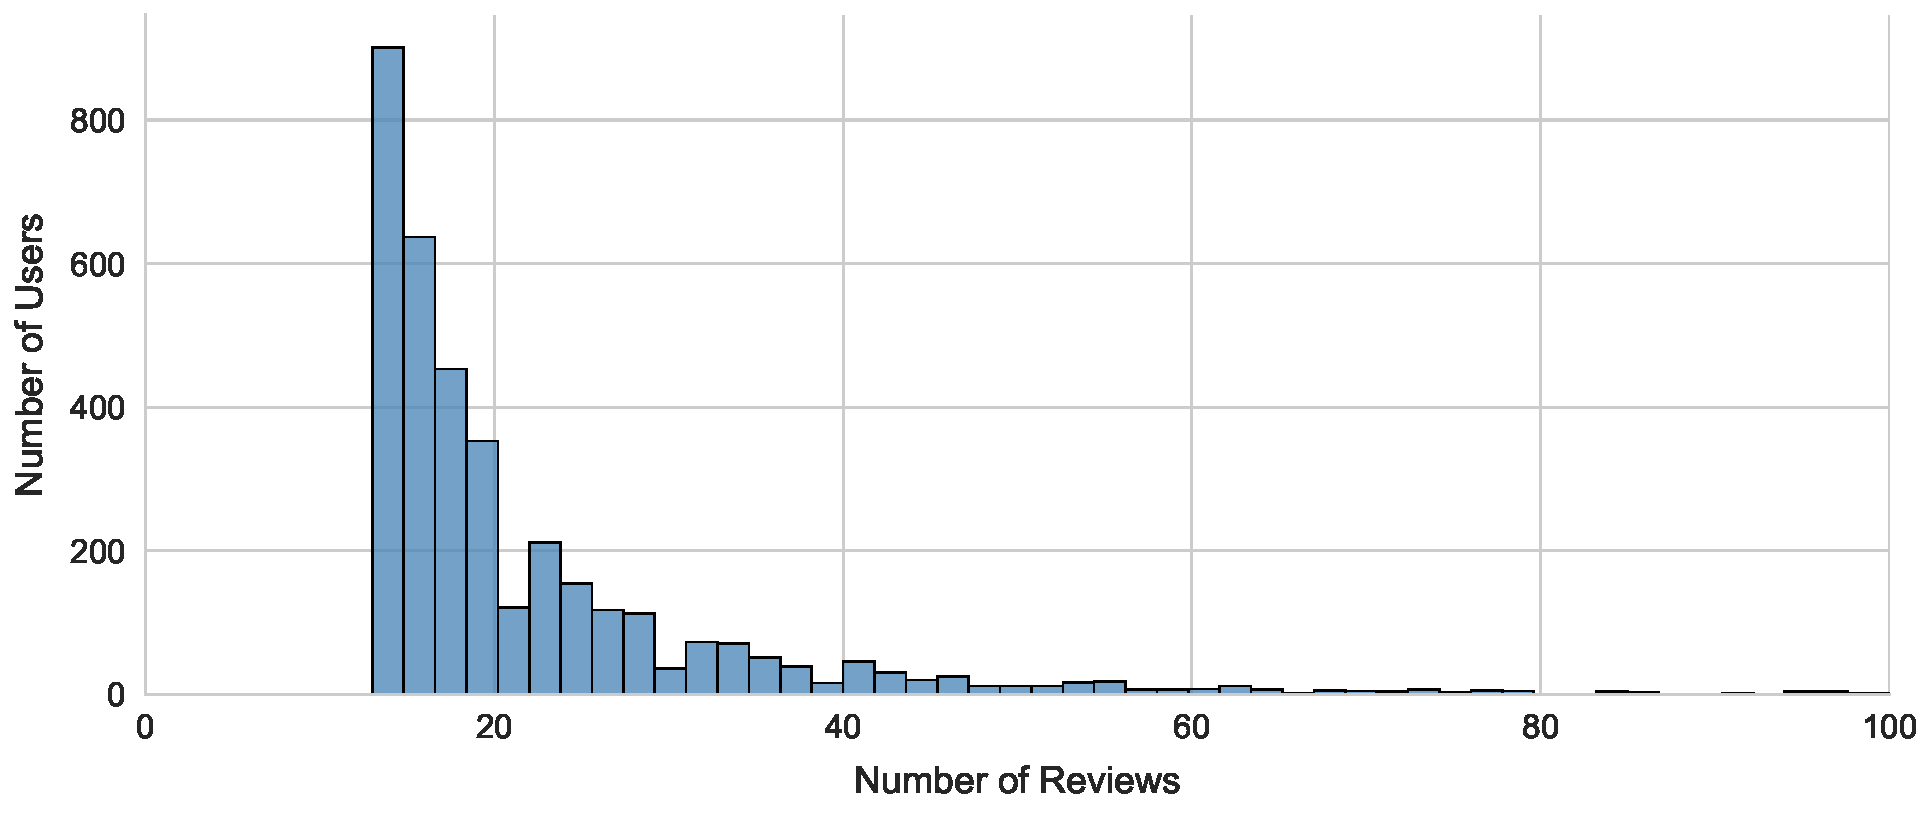
\includegraphics[width=0.9\textwidth]{Figures/reviews_per_user_distribution.pdf} % Adjust the width as needed
  \caption{Distribution of Reviews per Reviewer.}
  \label{fig:user review distribution}
\end{figure}

Additionally, a temporal analysis, shown in Figure \ref{fig:reviews per year}, illustrates an increasing trend in the number of reviews over time which illustrates an increasing trend in user engagement. Specifically, the line chart in Figure \ref{fig:reviews per year} displays the trend in the number of reviews per year from 6 to 2018. It is clear that the number of reviews has experienced exponential growth over the years. The review count remains relatively low until around 2010, after which there is a sharp increase, indicating a surge in user engagement on the platform. This trend of exponential growth is a common characteristic of user-generated content on digital platforms, reflecting the rapid adoption and increasing popularity of online shopping and product reviews \cite{alzoubi2022effect}. In 2017, the review count reaches its peak at just over 20 000, demonstrating the high level of user engagement during this period. However, there is a noticeable dip in the number of reviews in 2018, with the count dropping to just under 5000 reviews. This decline is not indicative of a decrease in user engagement but it is likely due to the dataset only containing reviews up until February 2018. Therefore, the data for 2018 is not complete, which explains the sudden drop.

\begin{figure}[ht]
  \centering
  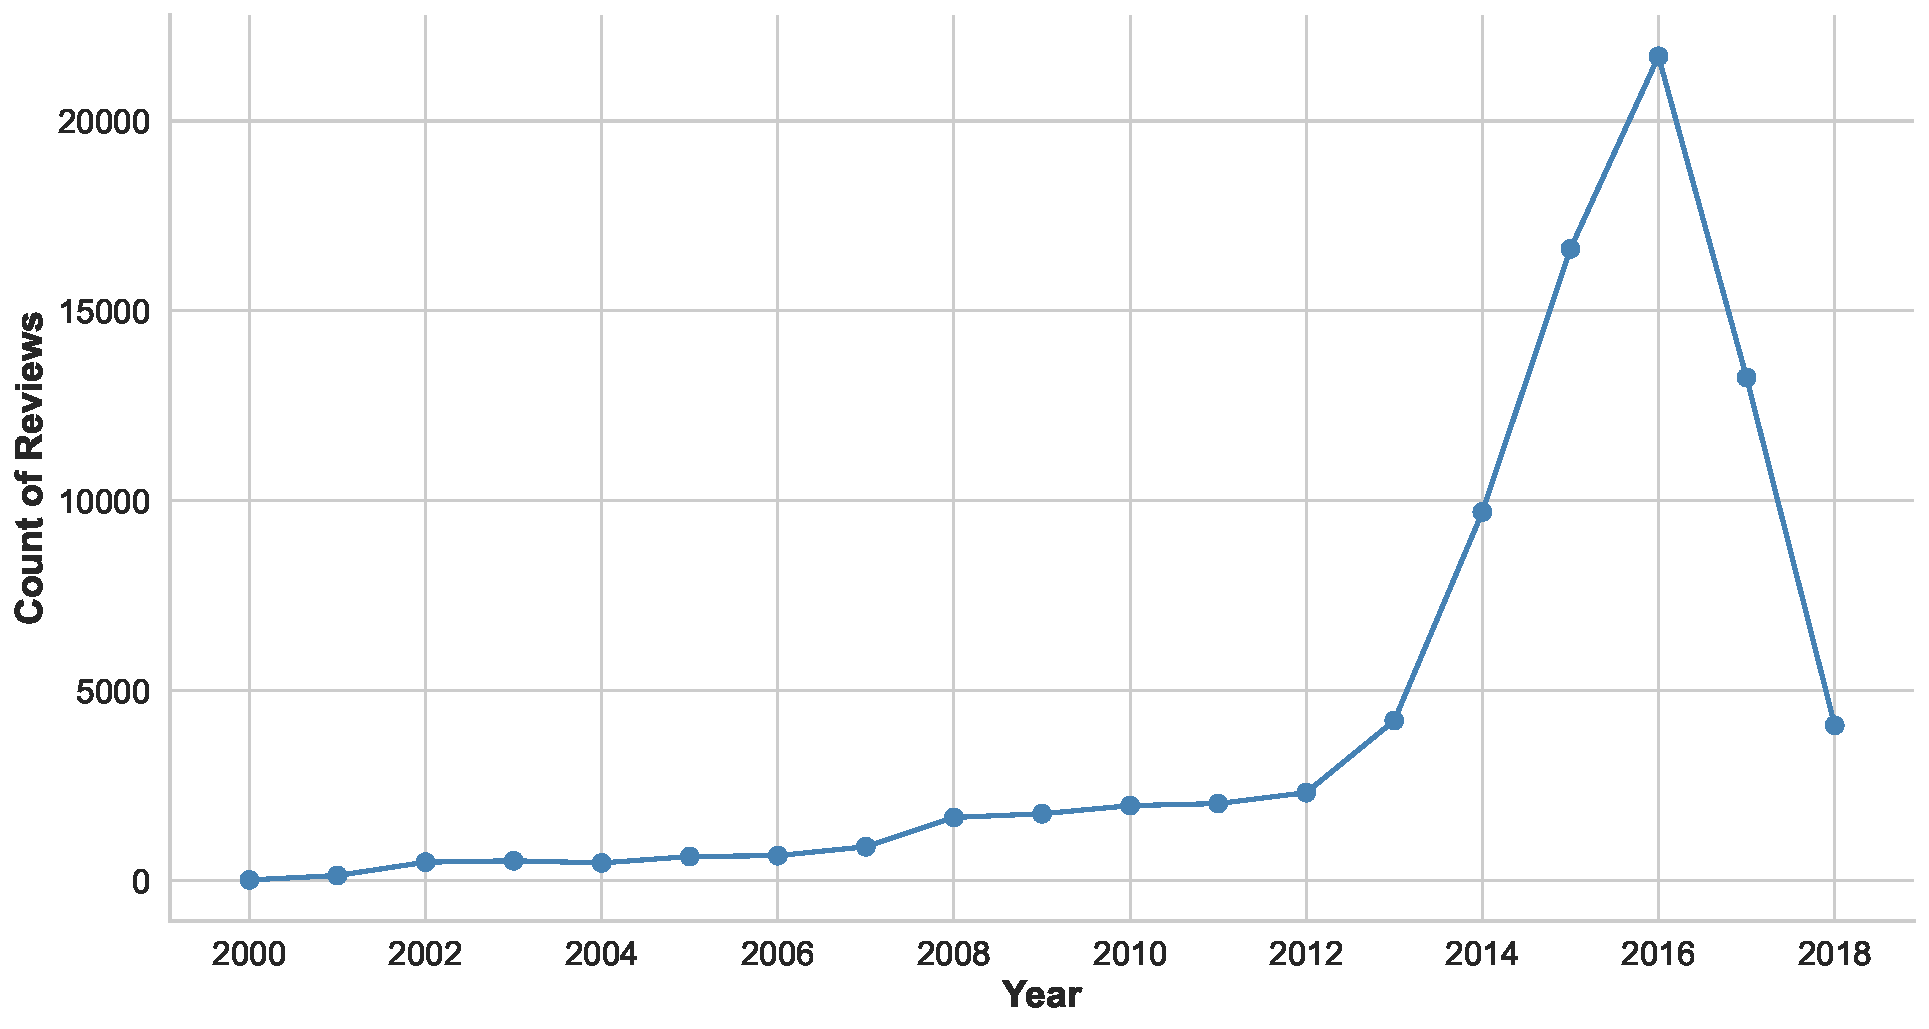
\includegraphics[width=0.9\textwidth]{Figures/reviews_per_year.pdf} % Adjust the width as needed
  \caption{Number of Reviews per Year.}
  \label{fig:reviews per year}
\end{figure}

These figures have provided valuable insights into the general user engagement, and in extension the temporal dynamics of user engagement in terms of review contribution on Amazon's e-commerce platform. Although the temporal aspect is not considered in this thesis, it is worthwhile showing to provide context on the dataset chosen. 

\subsection{Products}
\label{subsec:3 Products}

Similar to Figure \ref{fig:user review distribution}, we can look at the number of reviews per product. Analysing this is essential for shedding light on the dynamics and characteristics of the dataset that extend beyond individual user behaviors. Figure \ref{fig:product review distribution} illustrates the number of reviews per product. From the Figure, it is evident that a significant number of products have received fewer than 40 reviews, with a peak frequency observed for products with around 13 and 20 reviews. This suggests that while some products receive a high volume of reviews, the majority tend to have a relatively lower count.

Importantly, the figure aligns with our data subsetting process of ensuring that each product has at least 13 reviews. Again, this was done to alleviate the cold start problem, ensuring that there is sufficient interaction data for each product to generate reliable recommendations. Similar to Figure \ref{fig:user review distribution}, this product distribution is right skewed and the median number of reviews per product is 19. 

\begin{figure}[h]
  \centering
  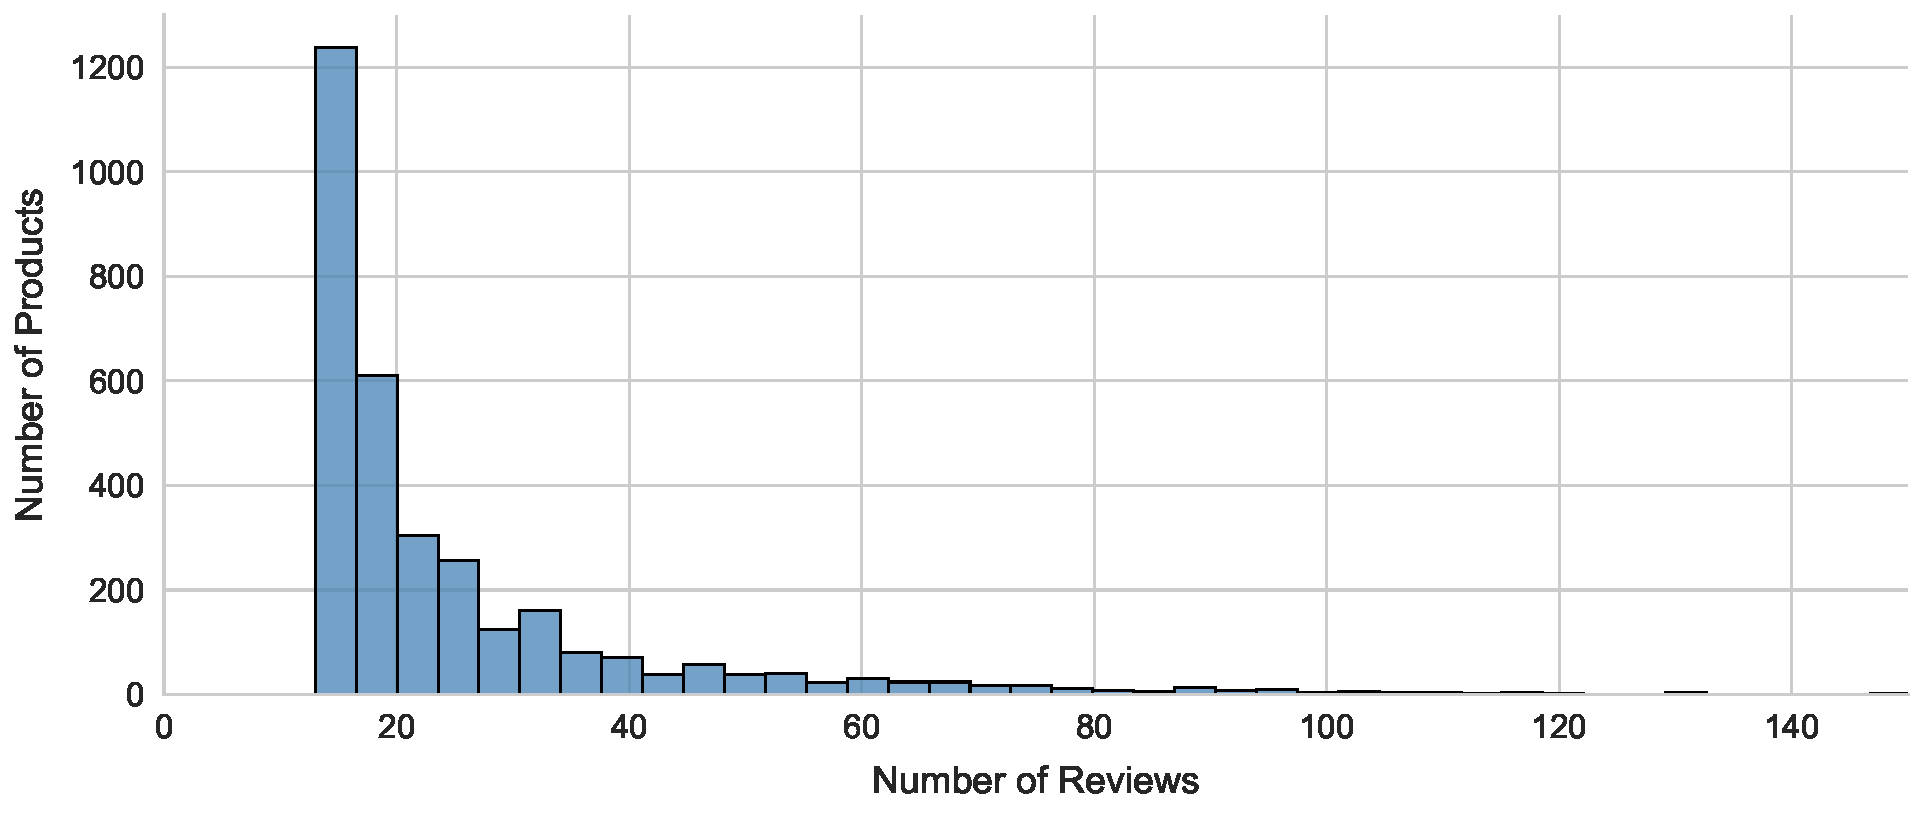
\includegraphics[width=0.9\textwidth]{Figures/reviews_per_product_distribution.pdf} % Adjust the width as needed
  \caption{Distribution of Reviews per Product.}
  \label{fig:product review distribution}
\end{figure}


\subsection{Ratings}
\label{subsec:3 Ratings}

We can also generate an overall picture of the dataset by looking at the distribution of ratings - allowing us to discern the user's general perception toward the products in our dataset. Figure \ref{fig:ratings distribution}, illustrates the the spread and central tendency of ratings. As mentioned in Section \ref{subsec:3 Amazon Review Dataset}, the rating scale is 1 to 5 for this Amazon Product Reviews dataset. From the Figure, it is clear that the majority of users have given a rating of 5, with the count exceeding 50 000 reviews. This suggests a high level of customer satisfaction, indicating that most users had positive experiences with the products they reviewed. On the other end of the spectrum, few users have given ratings of 1 and 2, with counts of 2000 and 3000 reviews respectively. This suggests that negative experiences are relatively rare among the users. Nevertheless, this scarcity could be indicative of two potential scenarios: either negative encounters are genuinely uncommon, or users may not be as prompt to express dissatisfaction compared to their enthusiasm in sharing positive experiences (\cite{chen2015augmenting};\cite{skalicky2015statistical})

\begin{figure}[h]
  \centering
  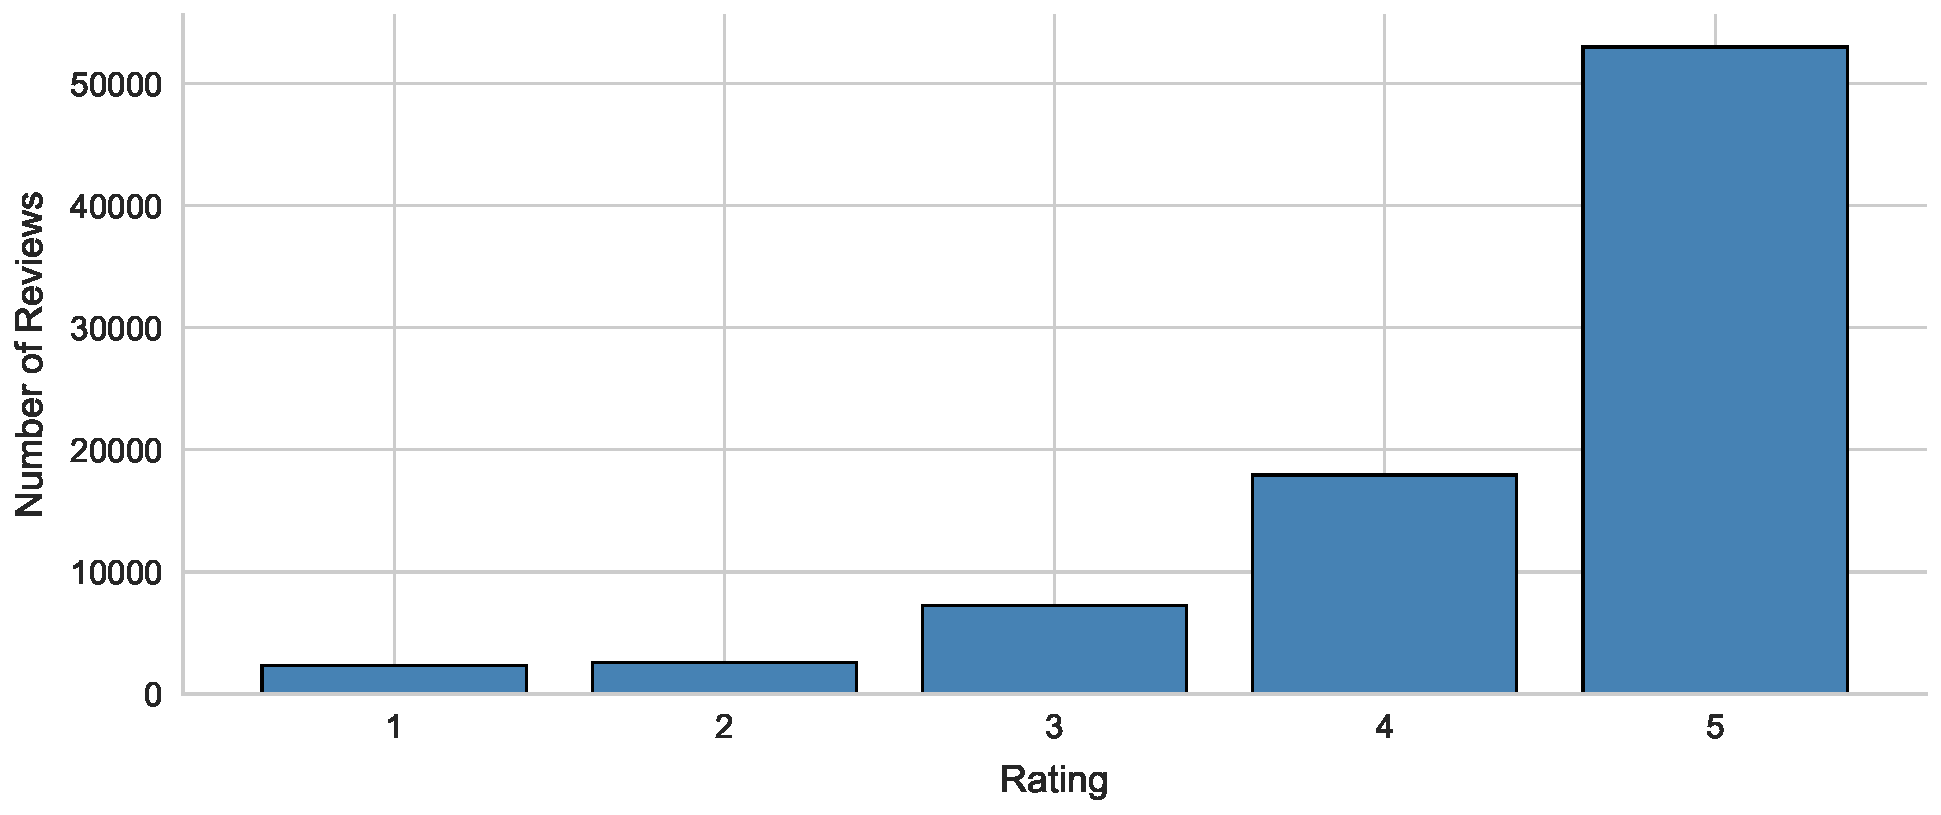
\includegraphics[width=0.9\textwidth]{Figures/rating_distribution.pdf} % Adjust the width as needed
  \caption{Distribution of Ratings from Users.}
  \label{fig:ratings distribution}
\end{figure}

Ultimately, understanding the distribution of user ratings is crucial for building and optimising our recommender system as it plays a large role in informing us of the potential user bias. We complement this Figure by looking at the the summary statistics in Table \ref{tab:rating summary}, for the ratings attribute which again reiterates how a large portion of the ratings are highly rated (5). Furthermore, the mean rating of 4.4 highlights the positive trend in the user feedback. Sentiment analysis scores could perhaps adjust for this bias, as they provide a more nuanced understanding of user preferences and opinions, which can potentially enhance the recommenders  ability to better capture the user's preferences and satisfaction with products and ultimately provide more accurate and relevant recommendations \cite{dang2021approach}.

\begin{table}[ht]
  \centering
  \begin{tabular}{l c}
      \hline
      \textbf{Statistic} & \textbf{Value} \\
      \hline
      Count & 83 139 \\
      Mean & 4.40 \\
      Standard Deviation & 0.97 \\
      Minimum & 1 \\
      25\% Percentile & 4 \\
      50\% Percentile & 5 \\
      75\% Percentile & 5 \\
      Maximum & 5 \\
      \hline
  \end{tabular}
  \caption{Summary Statistics of Ratings}
  \label{tab:rating summary}
\end{table}



\subsection{Review Text and Sentiments}
\label{subsec:3 Review Text}

Regarding the review, we have spent a considerable amount of time cleaning and preprocessing the this feature. We can now explore it, both from a lens of the textual content and the sentiments - the goal being to visualise and identify any patterns within the user reviews or sentiments. 

On average, we found that there are 127 words in each review. To supplement this, we visualise the distribution of the word count in Figure \ref{fig:distribution of word count}. From the Figure, it is clear that a majority of the reviews are relatively short, with most falling under 200 words - with large proportion of reviews containing below 100 words. This suggests that users typically prefer to leave concise feedback on products. Since we are looking at incorporating these reviews into NCF models, this could have several implications. Given that shorter reviews are more frequent, they might have a more significant impact on the prediction outcomes. However, shorter reviews might not always provide comprehensive insights into a user’s preferences or experiences, as they might lack detailed descriptions or explanations. On the other hand, longer reviews, although less frequent, might offer more detailed insights into a user’s preferences, potentially enhancing the accuracy of the recommendations. However, they might also introduce noise into the model due to the increased likelihood of off-topic content or unnecessary details. A potential outcome of this is that the model might be biased towards shorter reviews, as they are more frequent \cite{srifi2020recommender}. This shall be explored further in the Chapter \ref{Chapter5} - the results.

\begin{figure}[h]
  \centering
  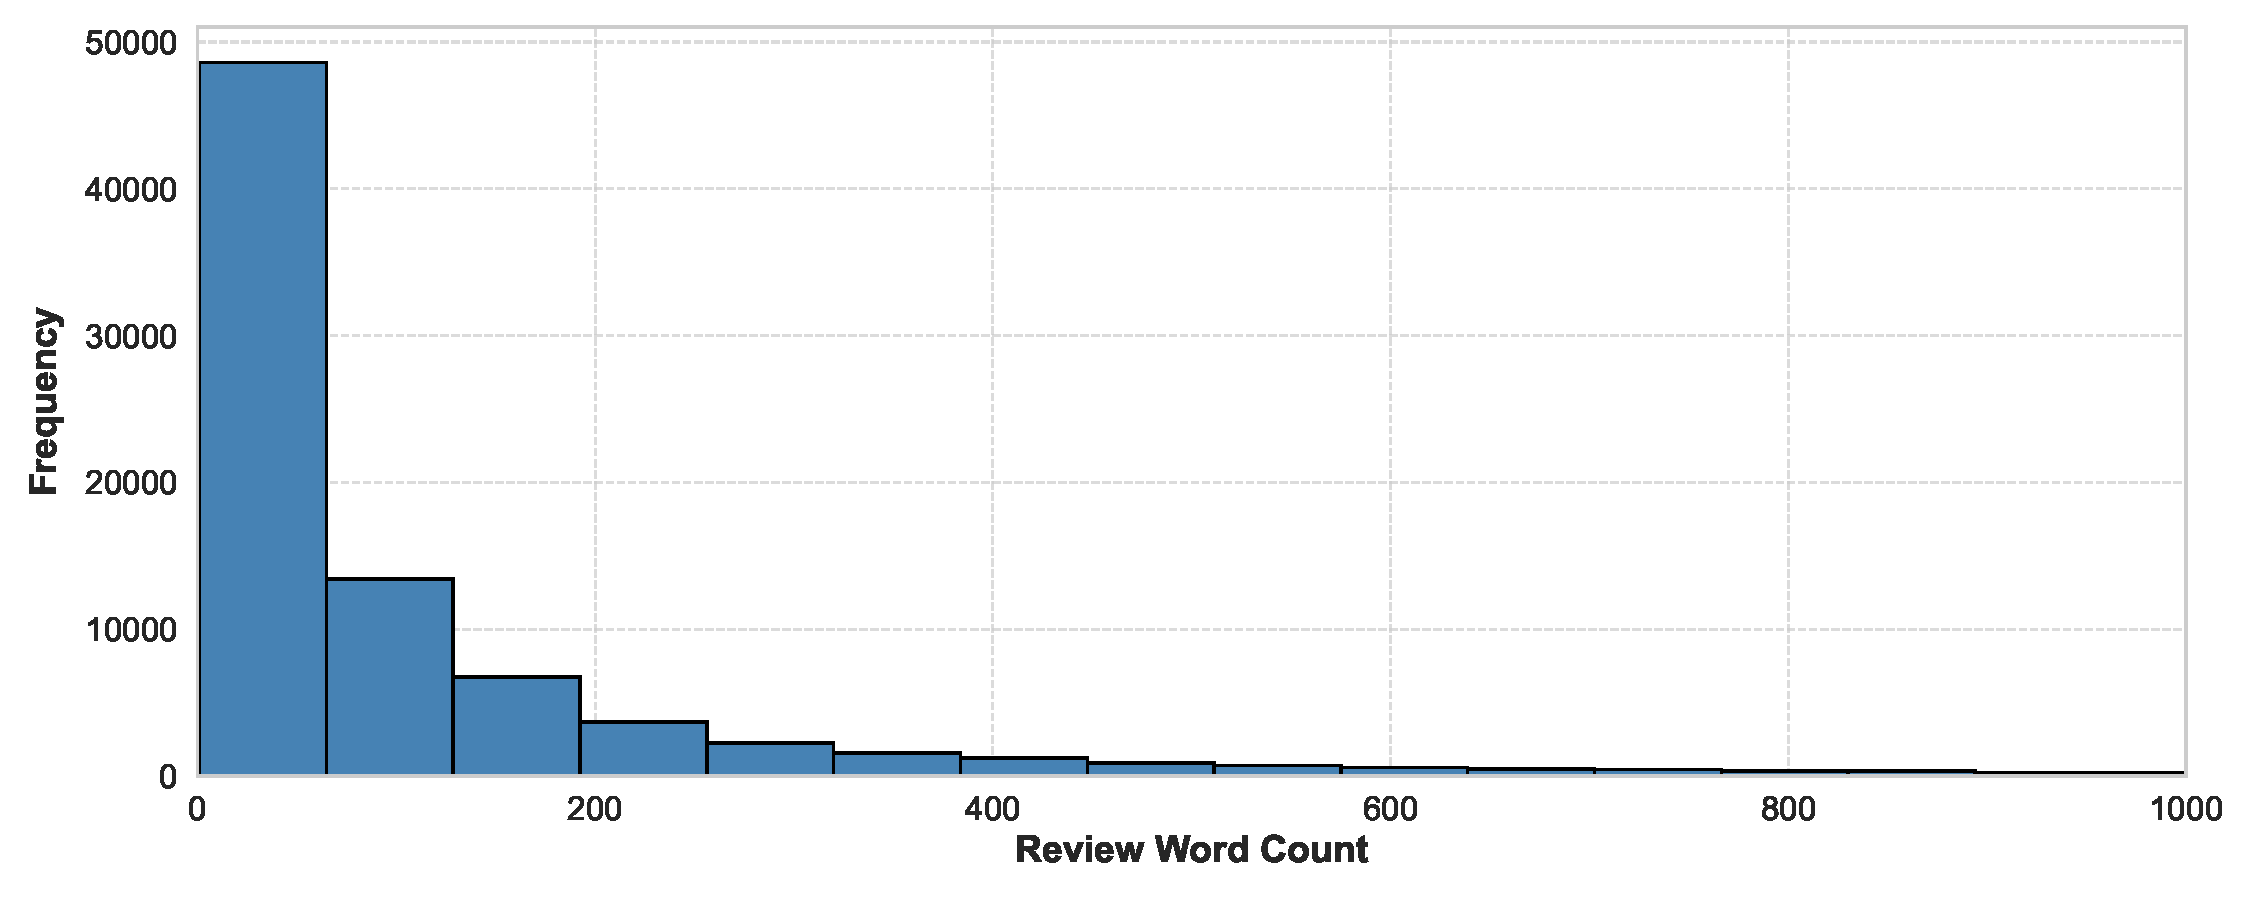
\includegraphics[width=0.9\textwidth]{Figures/distribution_of_review_word_count.pdf} % Adjust the width as needed
  \caption{Distribution of Review Word Count.}
  \label{fig:distribution of word count}
\end{figure}

Using the review text we can also explore the prevalence of specific phrases or consecutive words, commonly known as $n$-grams, where $n$ is the number of words \cite{mcauley2013hidden}. In Figure \ref{fig:n-grams}, we specifically examine the top 10 frequently occurring consecutive tri-grams (Figure \ref{fig:tri-grams}) and four-grams (Figure \ref{fig:four-grams}). This analysis provides insights into the distinctive linguistic structures that frequently appear in the reviews, improving our understanding of the language dynamics within the dataset.

\begin{figure}[h]
  \centering
  \begin{subfigure}{0.48\textwidth}
      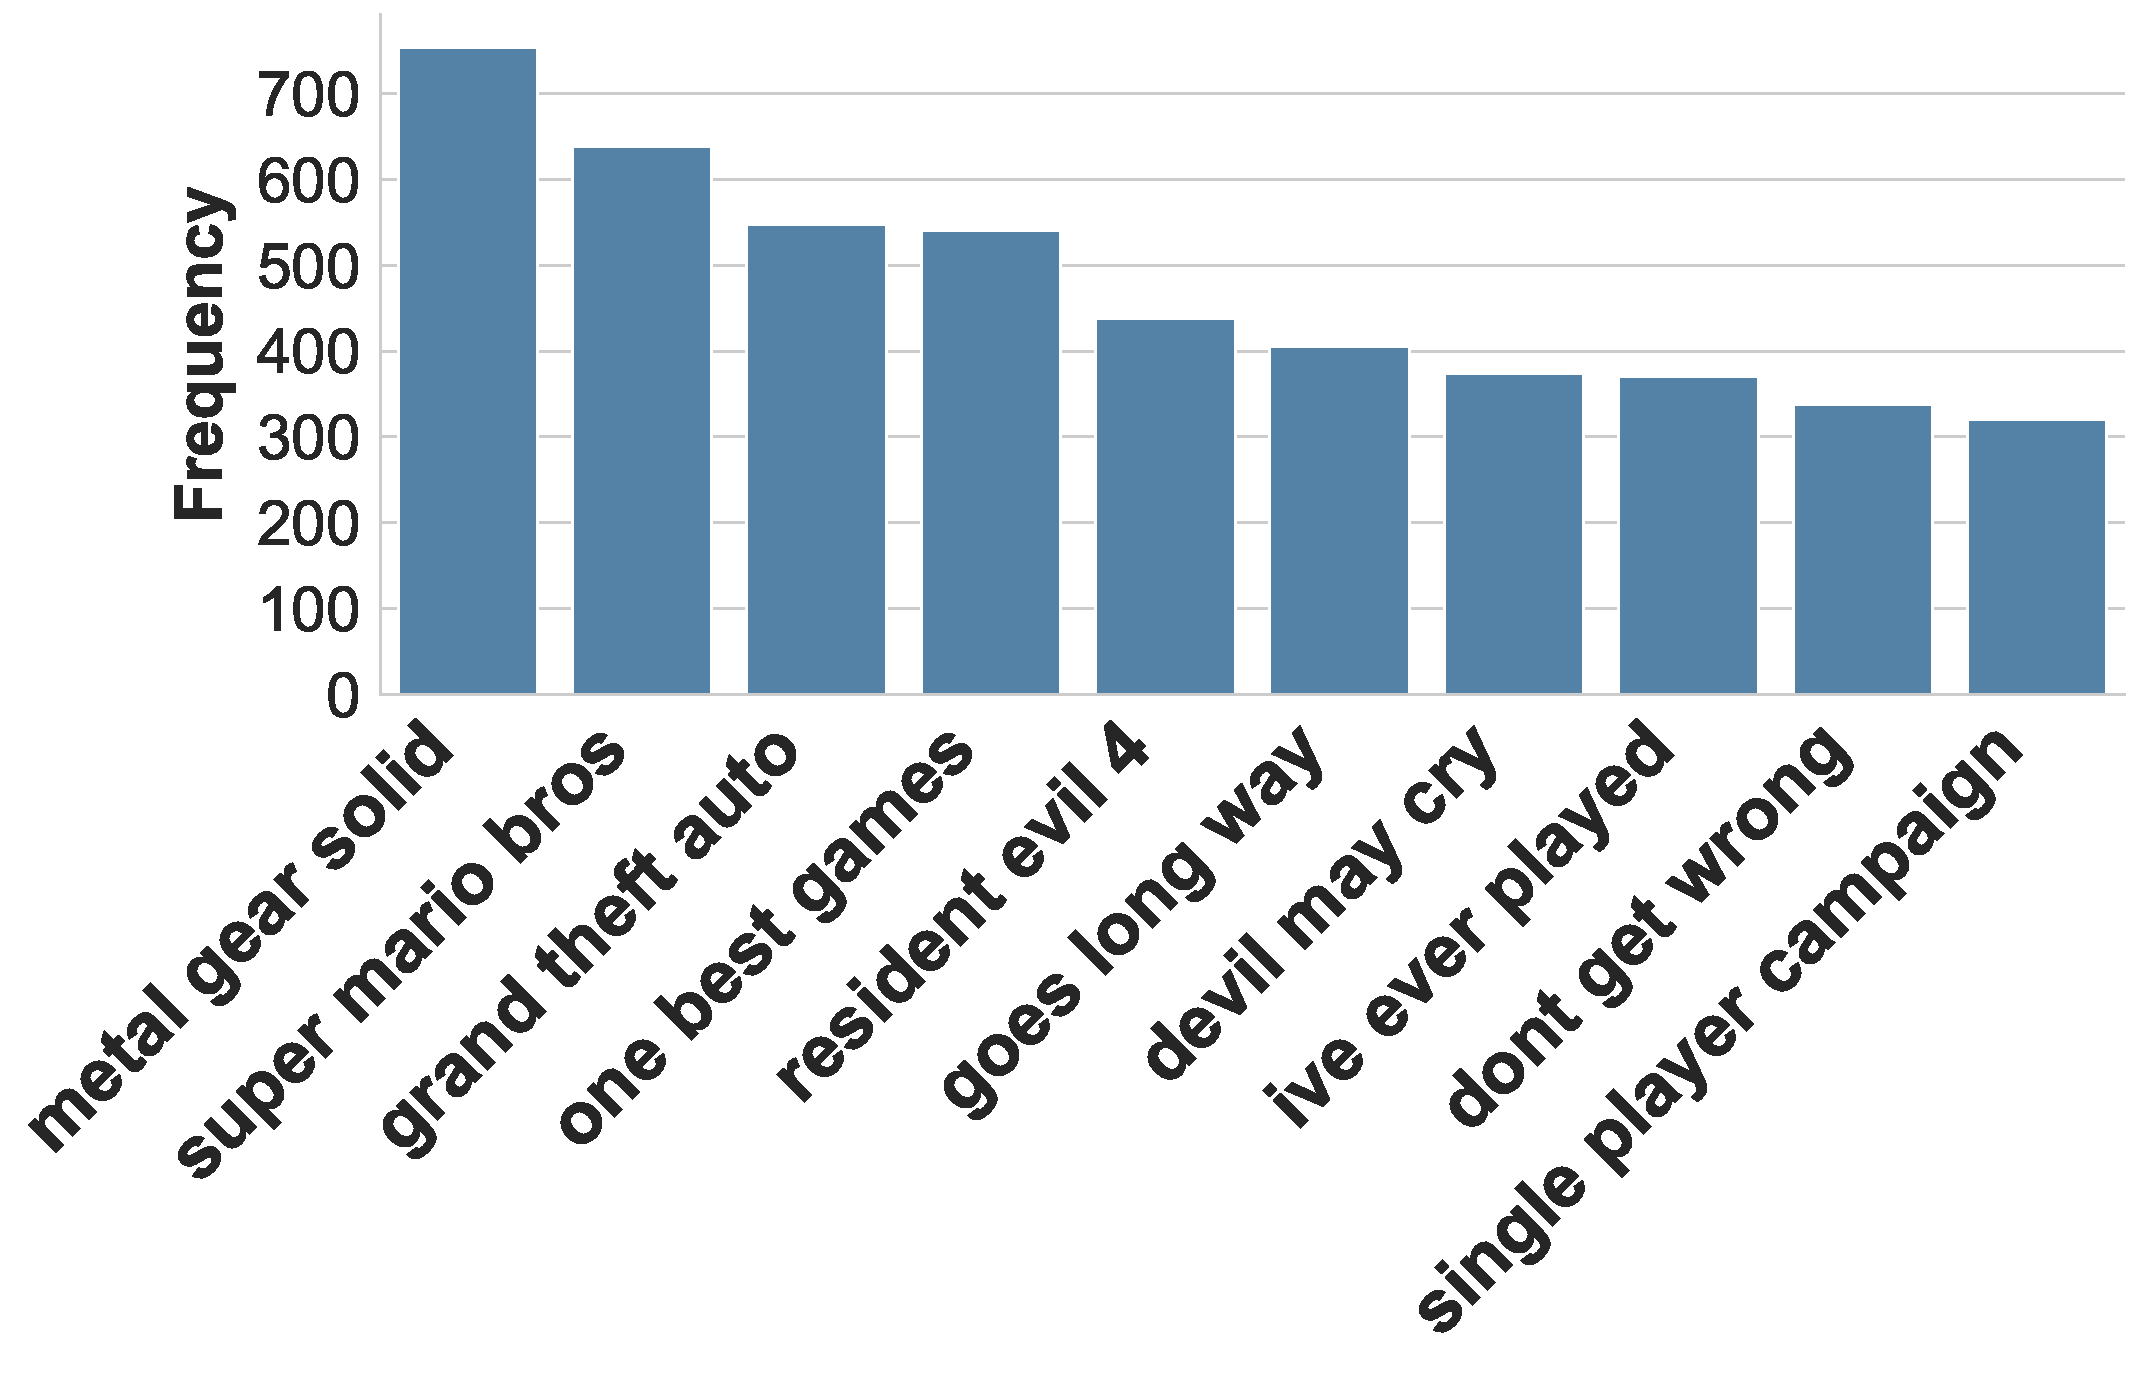
\includegraphics[width=\textwidth]{Figures/trigrams.pdf} % Adjust the file path and width as needed
      \caption{Tri-gram}
      \label{fig:tri-grams}
  \end{subfigure}
  \hfill
  \begin{subfigure}{0.48\textwidth}
      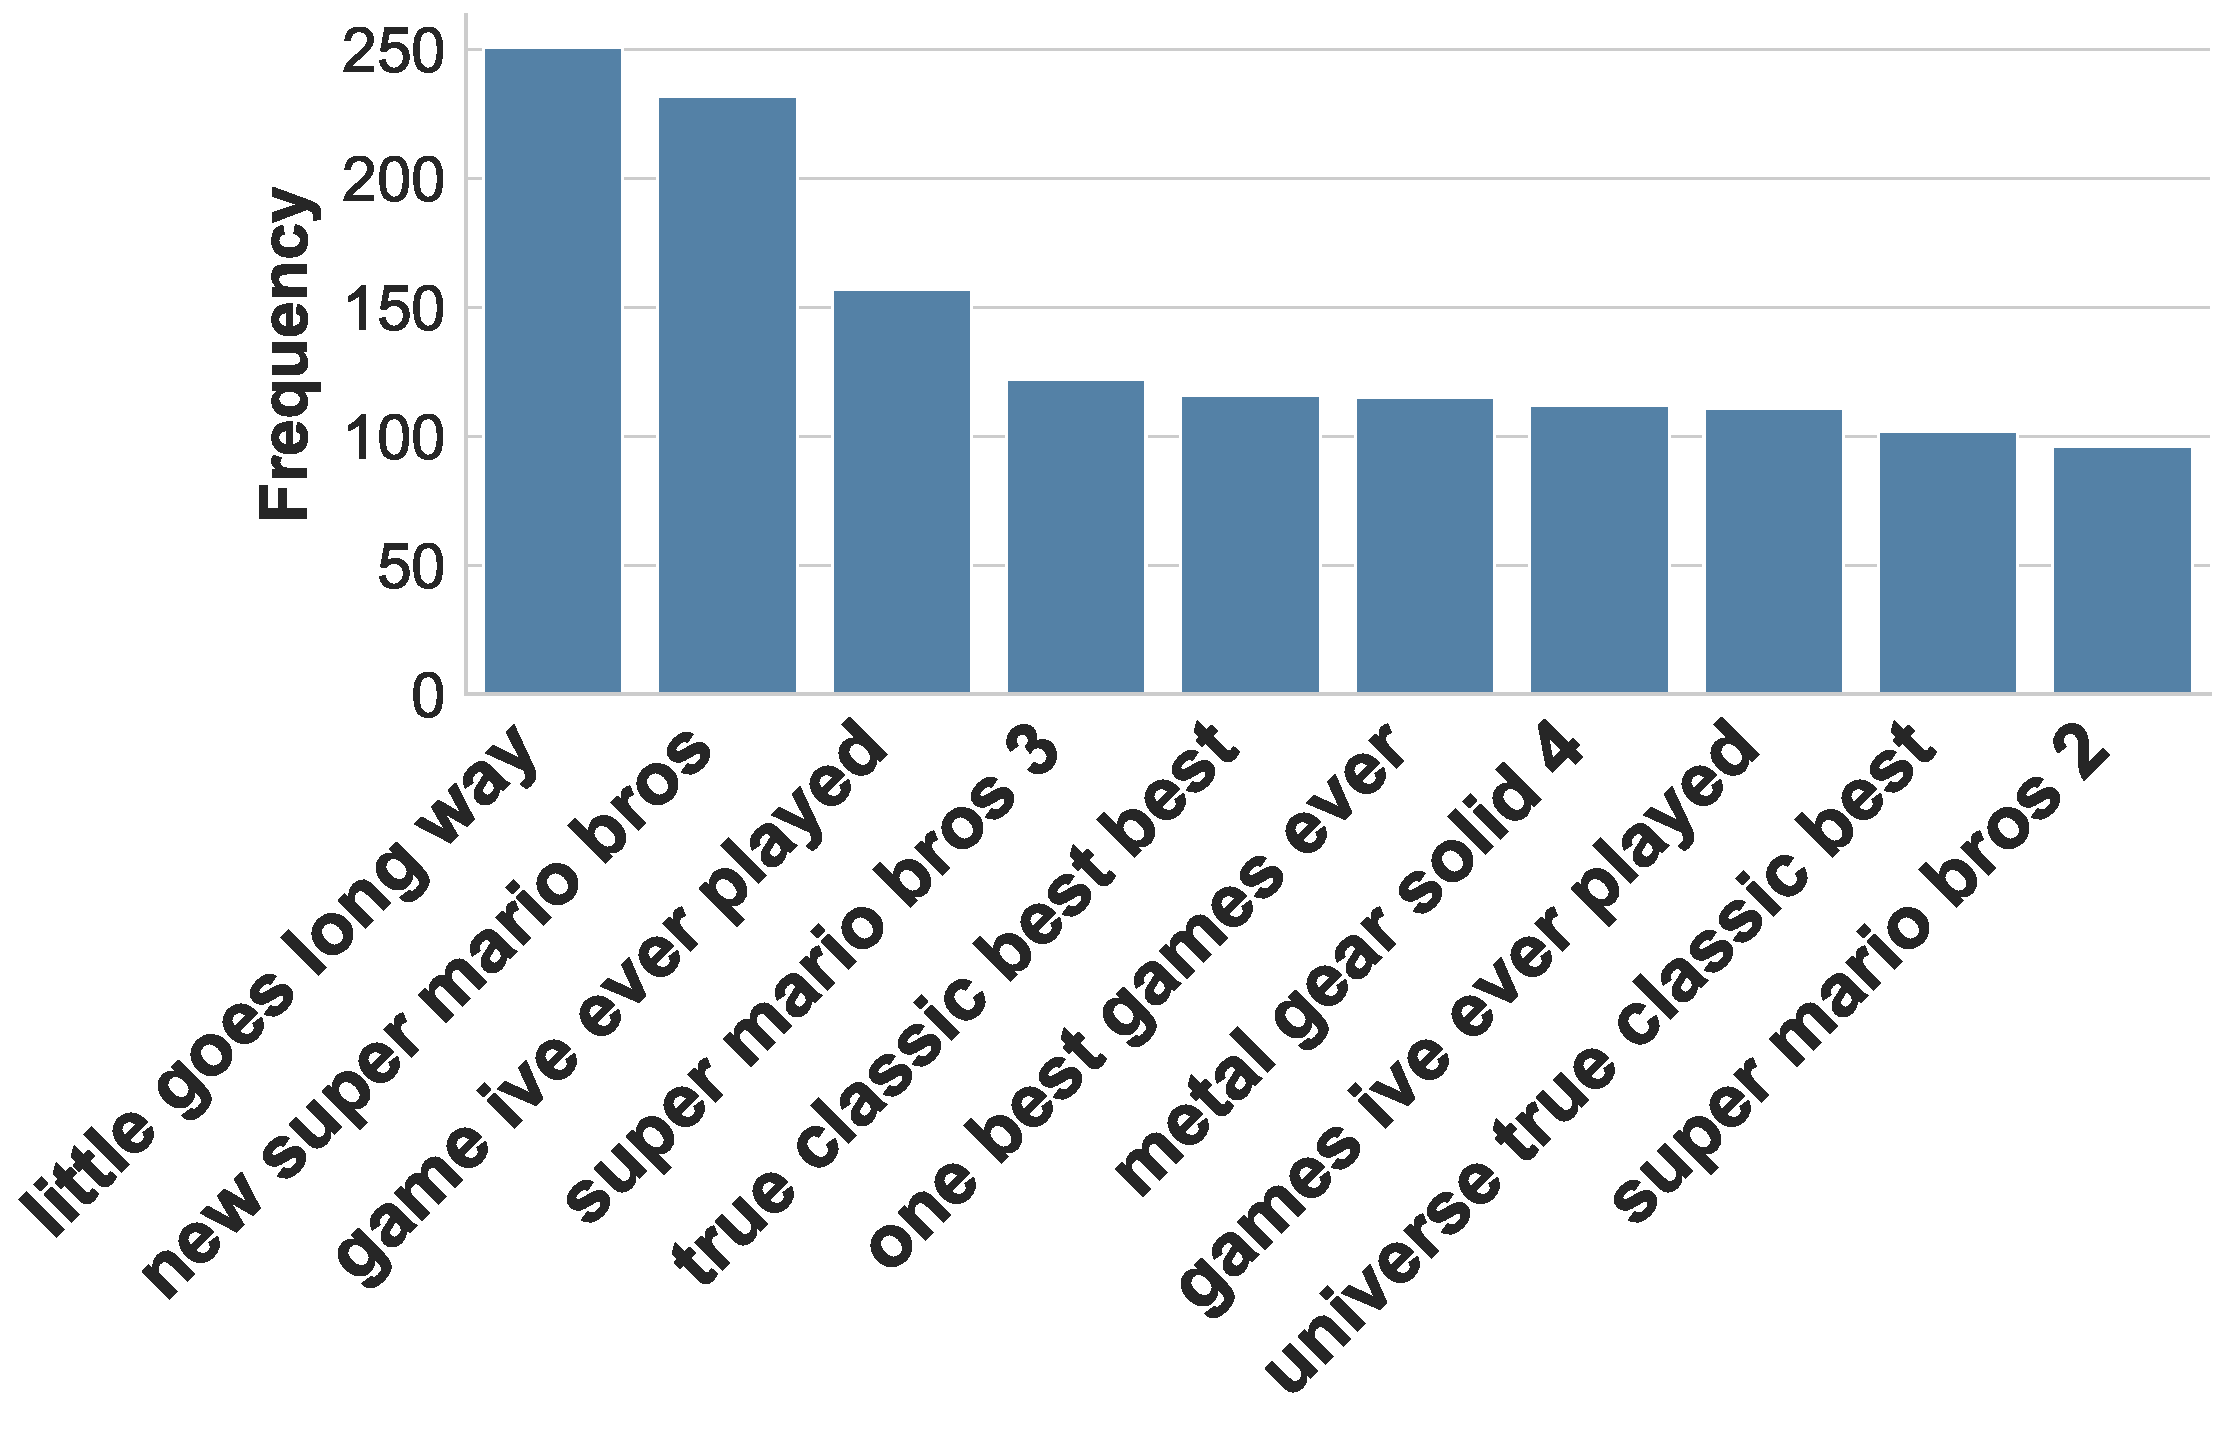
\includegraphics[width=\textwidth]{Figures/fourgrams.pdf} % Adjust the file path and width as needed
      \caption{Four-gram}
      \label{fig:four-grams}
  \end{subfigure}
  \caption{Top 10 N-grams in Review Text from Users}
  \label{fig:n-grams}
\end{figure}

From the Figure \ref{fig:n-grams}, it is clear that phrases like “metal gear solid”, “grand theft auto”, and “super mario bros” are among the most frequent tri-grams. These tri-grams appear to be related to popular video game titles, suggesting that our dataset includes a significant amount of reviews for these games or rather, users frequently mention these games in their reviews. This could be indicative of the popularity of these games among users. Other tri-grams like “one best games”, “can’t go wrong”, and “goes long way” could be common phrases users employ to express their positive experiences or high regard for a product.  We find similar results when we look at the four-grams (Figure \ref{fig:four-grams}) where some of the phrases are  “little goes long way”, “now super mario bros”, and “one best games ever” are among the most frequently used. 

These $N$-grams are useful in text analysis as they provide context that individual words might not. By considering sequences of words (like tri-grams and four-grams), we can capture more meaningful phrases that often occur in our text data. This can help in understanding common themes or topics in our reviews \cite{collins2019document}. Furthermore, in the context of our recommender system, these $n$-grams can provide valuable insights into the aspects that users frequently discuss or value in products \cite{srifi2020recommender}. However, it’s important to note that while $n$-grams can capture local context (i.e., within the $n$-gram), they might not capture the overall sentiment of a review if it’s expressed through complex or long-range dependencies between words. Techniques like sentiment analysis, which we employed, are more effective in capturing the overall sentiment of a review, as they consider the entire review text \cite{collins2019document}.

To that end, we can also explore the distribution of the sentiment scores from from each of the three sentiment analysis lexicon-based methods in Figure \ref{fig:comparison_sentiments}. From Figure \ref{fig:comparison_sentiments}, it is clear that the distribution of sentiment scores from AFINN (Figure \ref{fig:afinn sentiment distribution}) and BING (Figure \ref{fig:bing sentiment distribution}) are similar, while the distribution of sentiment scores from VADER (Figure \ref{fig:vader sentiment distribution}) is distinct. For AFINN and BING, their distributions are uni-modal and skewed to the right, with most sentiment scores concentrated around 0. This suggests that these sentiment analysis techniques tends to classify a significant portion of the reviews as neutral. In contrast to Figures \ref{fig:bing sentiment distribution} and \ref{fig:afinn sentiment distribution}, the sentiment score distribution for VADER (Figure \ref{fig:vader sentiment distribution}) illustrates sentiment scores not uniformly distributed. Most of the sentiment scores are clustered around 0 and 1, indicating that most reviews are either neutral or positive. There is a significant spike in frequency close to the 1.00 score, suggesting a large volume of highly positive sentiments in the reviews. Given that we have spikes at 0, 1 scores, as well as some reviews classified negatively (as shown in Figure \ref{fig:vader sentiment distribution}), we find that the distribution of VADER sentiments illustrates that this technique is capturing both the positive, neutral, and negative sentiments in our review data, albeit with a higher frequency of positive sentiments. We expect this behaviour since the distribution of ratings (as shown in Figure \ref{fig:ratings distribution}) is heavily skewed towards the higher ratings.

As we mentioned in Section \ref{subsec:3 Sentiment Analysis} we opted for VADER as it held the strongest correlation with the user ratings. This decision seems well-supported as VADER, unlike AFINN and BING, captures a wider range of sentiments (as shown from Figure \ref{fig:vader sentiment distribution}), which could lead to a more nuanced understanding of user opinions. This can be particularly useful for our recommender system as it can help in capturing more detailed user preferences, potentially enhancing the accuracy of our recommendations \cite{dang2021approach}. 

\begin{figure}[h]
  \centering
  \begin{subfigure}{0.49\textwidth} % Adjust the width based on the number of figures and desired spacing
      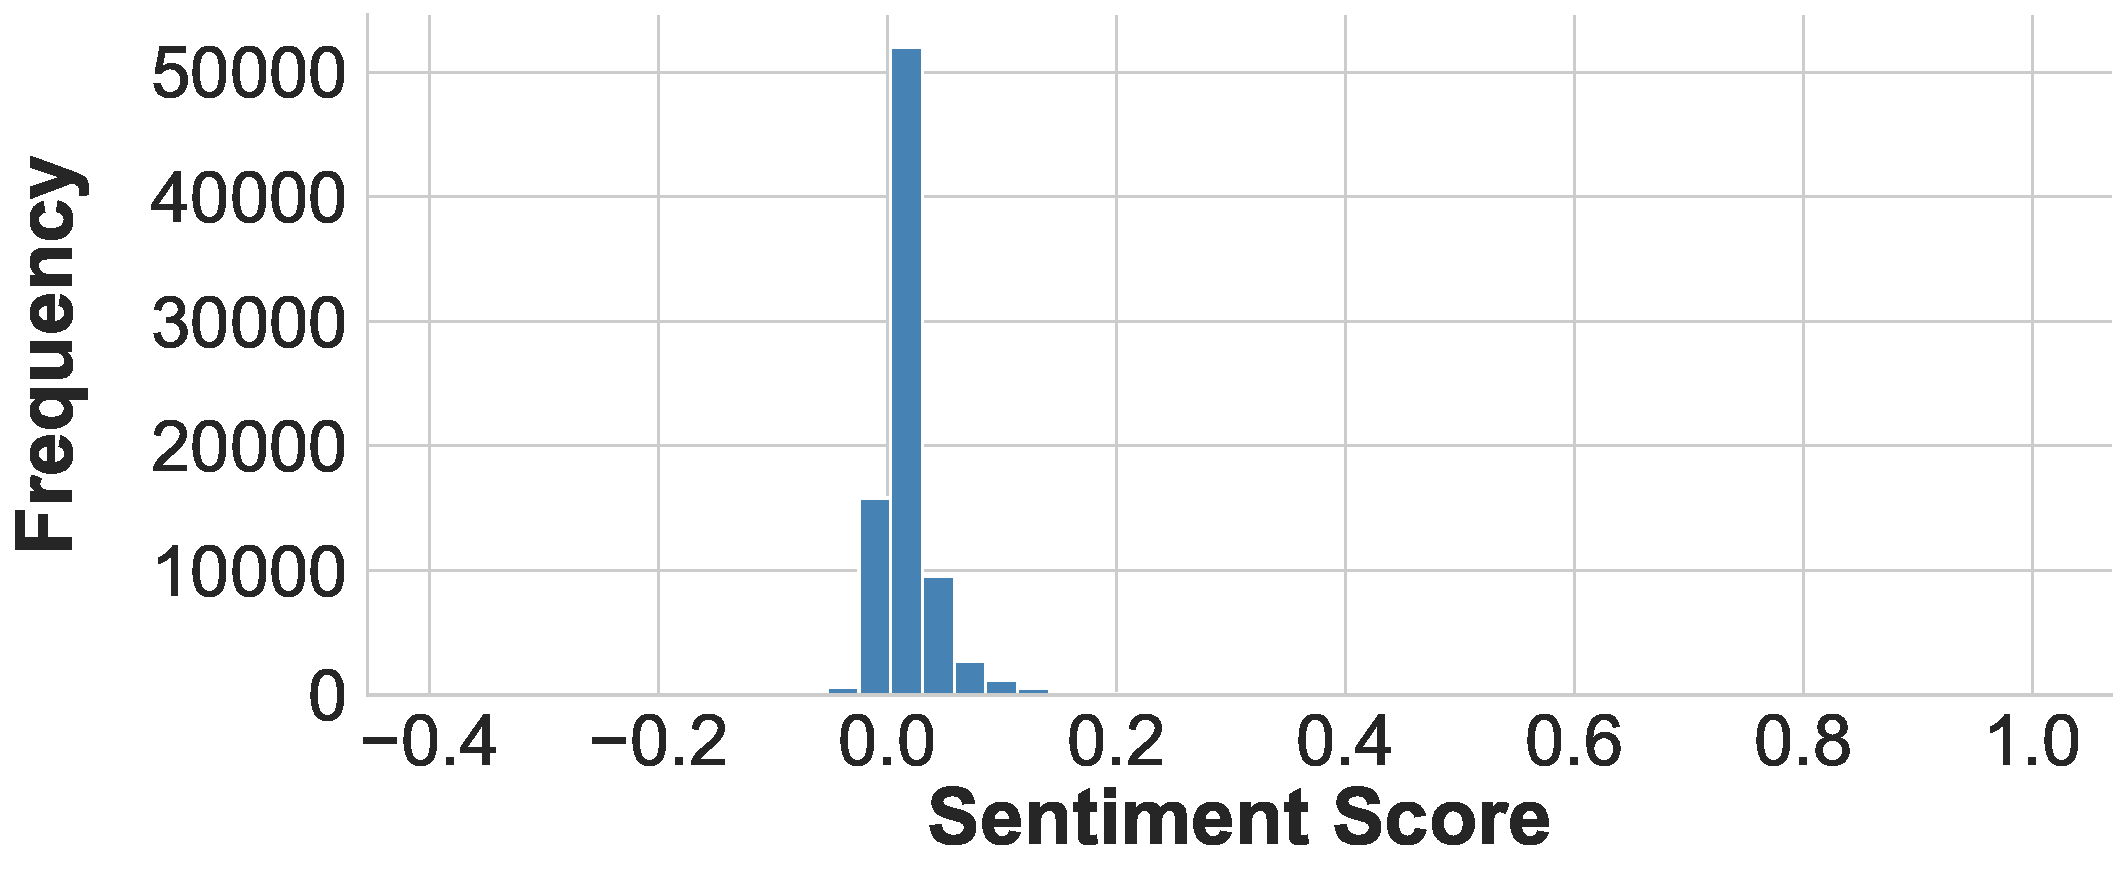
\includegraphics[width=\textwidth]{Figures/distribution_afinn.pdf} % Adjust the file path and width as needed
      \caption{AFINN}
      \label{fig:afinn sentiment distribution}
  \end{subfigure}
  \hfill
  \begin{subfigure}{0.49\textwidth} % Adjust the width based on the number of figures and desired spacing
      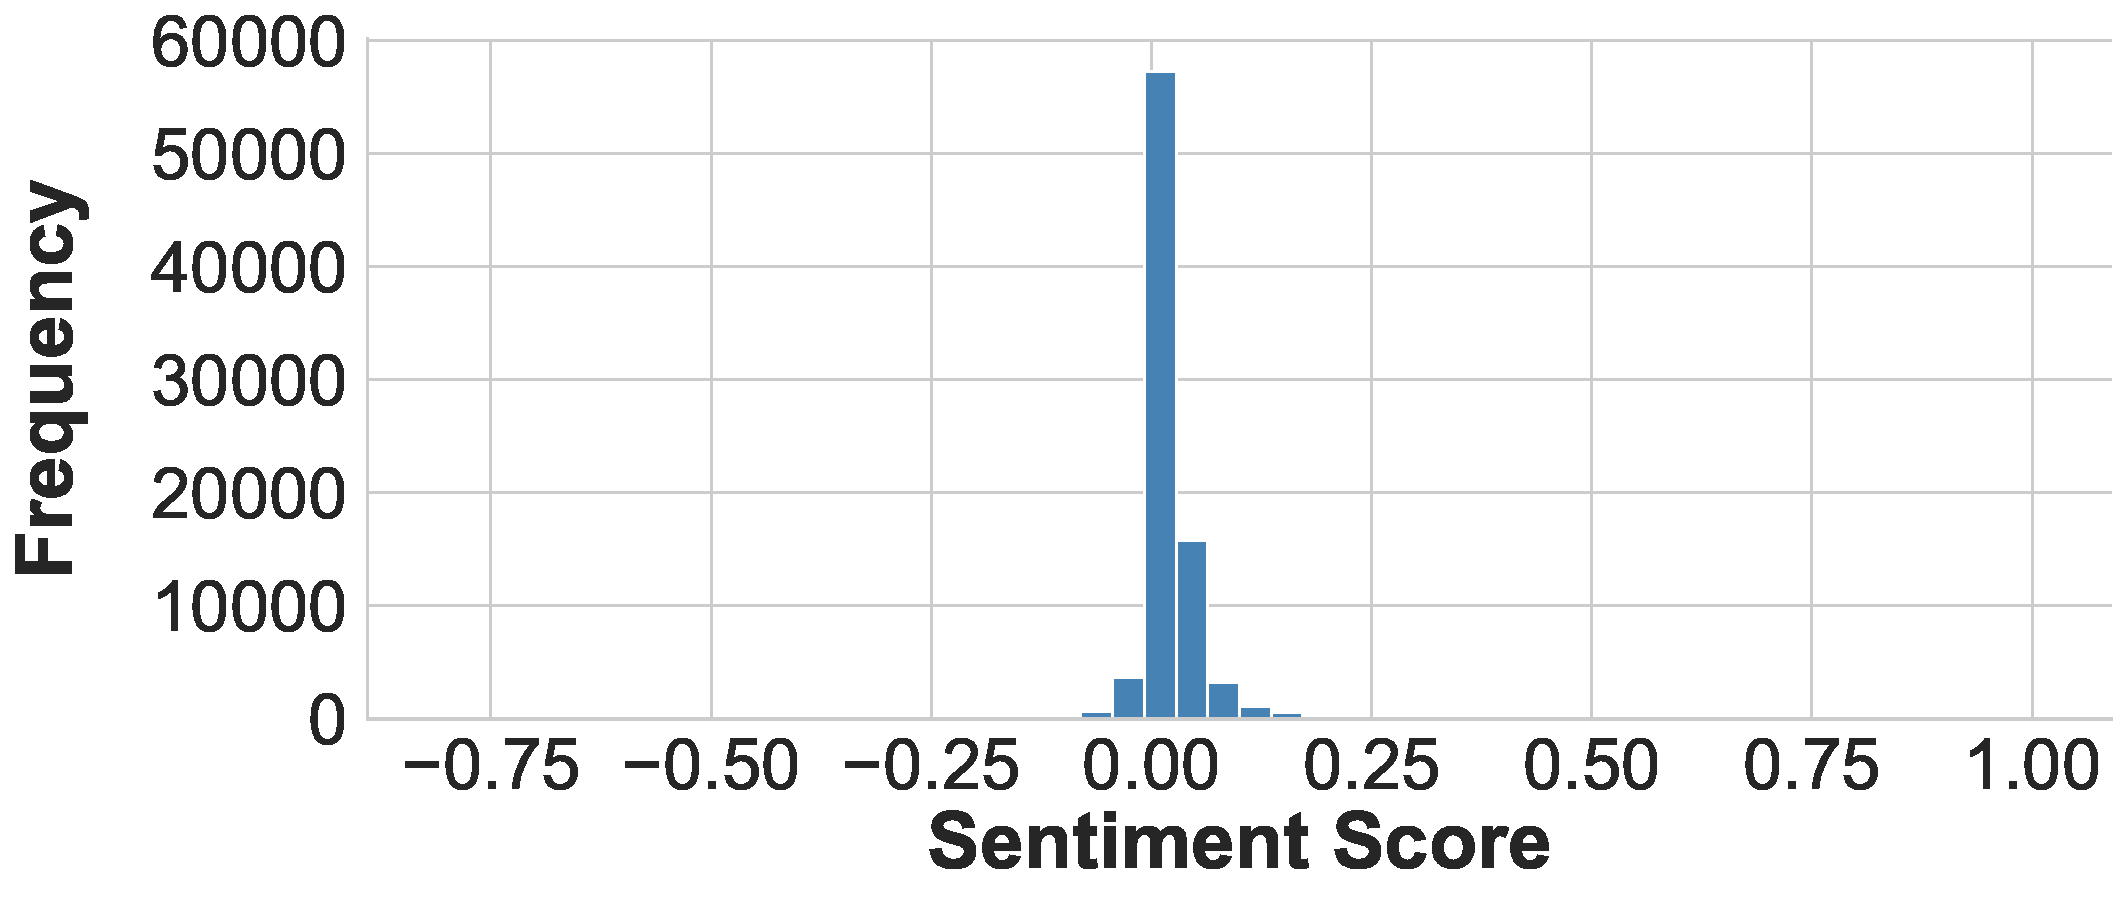
\includegraphics[width=\textwidth]{Figures/distribution_bing.pdf} % Add the path to the third figure
      \caption{BING} % Add a caption for the third figure
      \label{fig:bing sentiment distribution} % Add a label for the third figure
  \end{subfigure}
  \vskip\baselineskip % Add vertical space between rows
  \begin{subfigure}{0.999\textwidth} % Adjust the width based on the number of figures and desired spacing
      \centering
      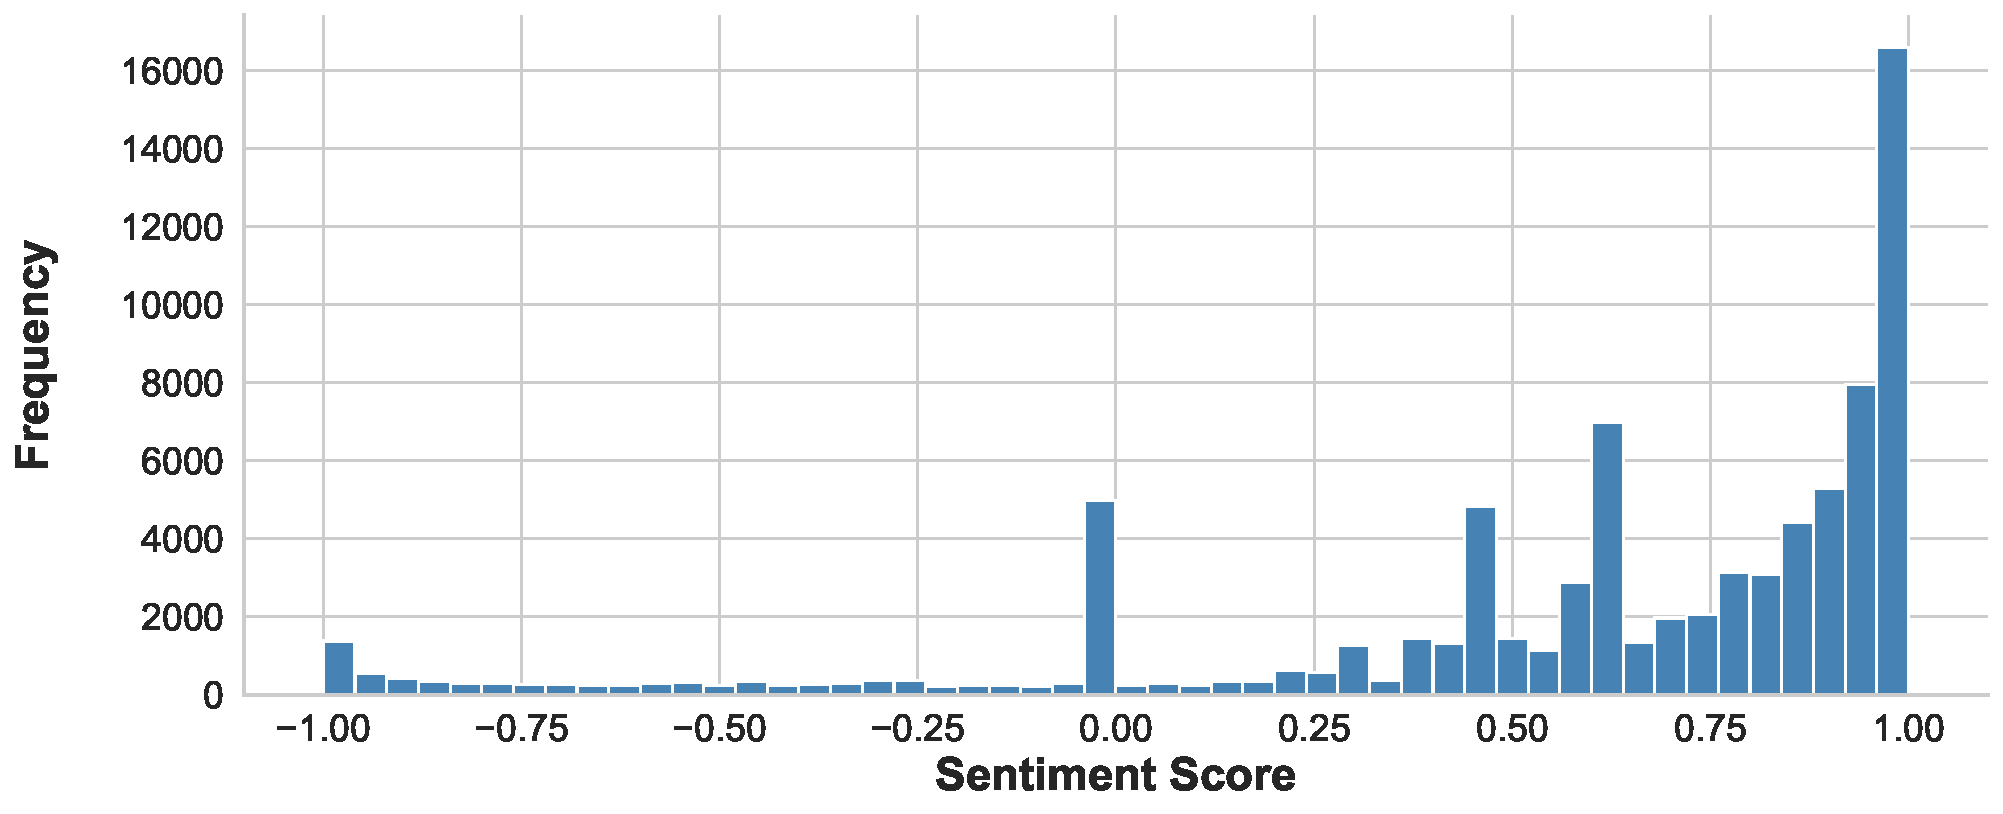
\includegraphics[width=0.9\textwidth]{Figures/distribution_vader.pdf} % Adjust the file path and width as needed
      \caption{VADER}
      \label{fig:vader sentiment distribution}
  \end{subfigure}
  \caption{Distribution of Sentiment Scores for AFINN, BING, and VADER algorithms.} % Update the caption accordingly
  \label{fig:comparison_sentiments}
\end{figure}



In Figures \ref{fig:top 10 products sentiments} and \ref{fig:bottom 10 products sentiments}, we identify the the top 10 products and bottom 10 products based on their average sentiment scores. We see that the top products have similar mean sentiment scores. In contrast, there is a clearer difference between the bottom 10 products. Additionally, Tables \ref{tab:top 10 products statistics} and \ref{tab:bottom 10 products statistics} illustrates that the ratings for the top 10 and bottom 10 products (by sentiment) line up quite well. This is indicative of a consistent correlation between product (VADER) sentiment and user ratings, suggesting that products with higher sentiment scores tend to receive more positive ratings, while those with lower sentiment scores align with lower ratings. 

\begin{figure}[h]
  \centering
  \begin{subfigure}{\textwidth}
    \centering
    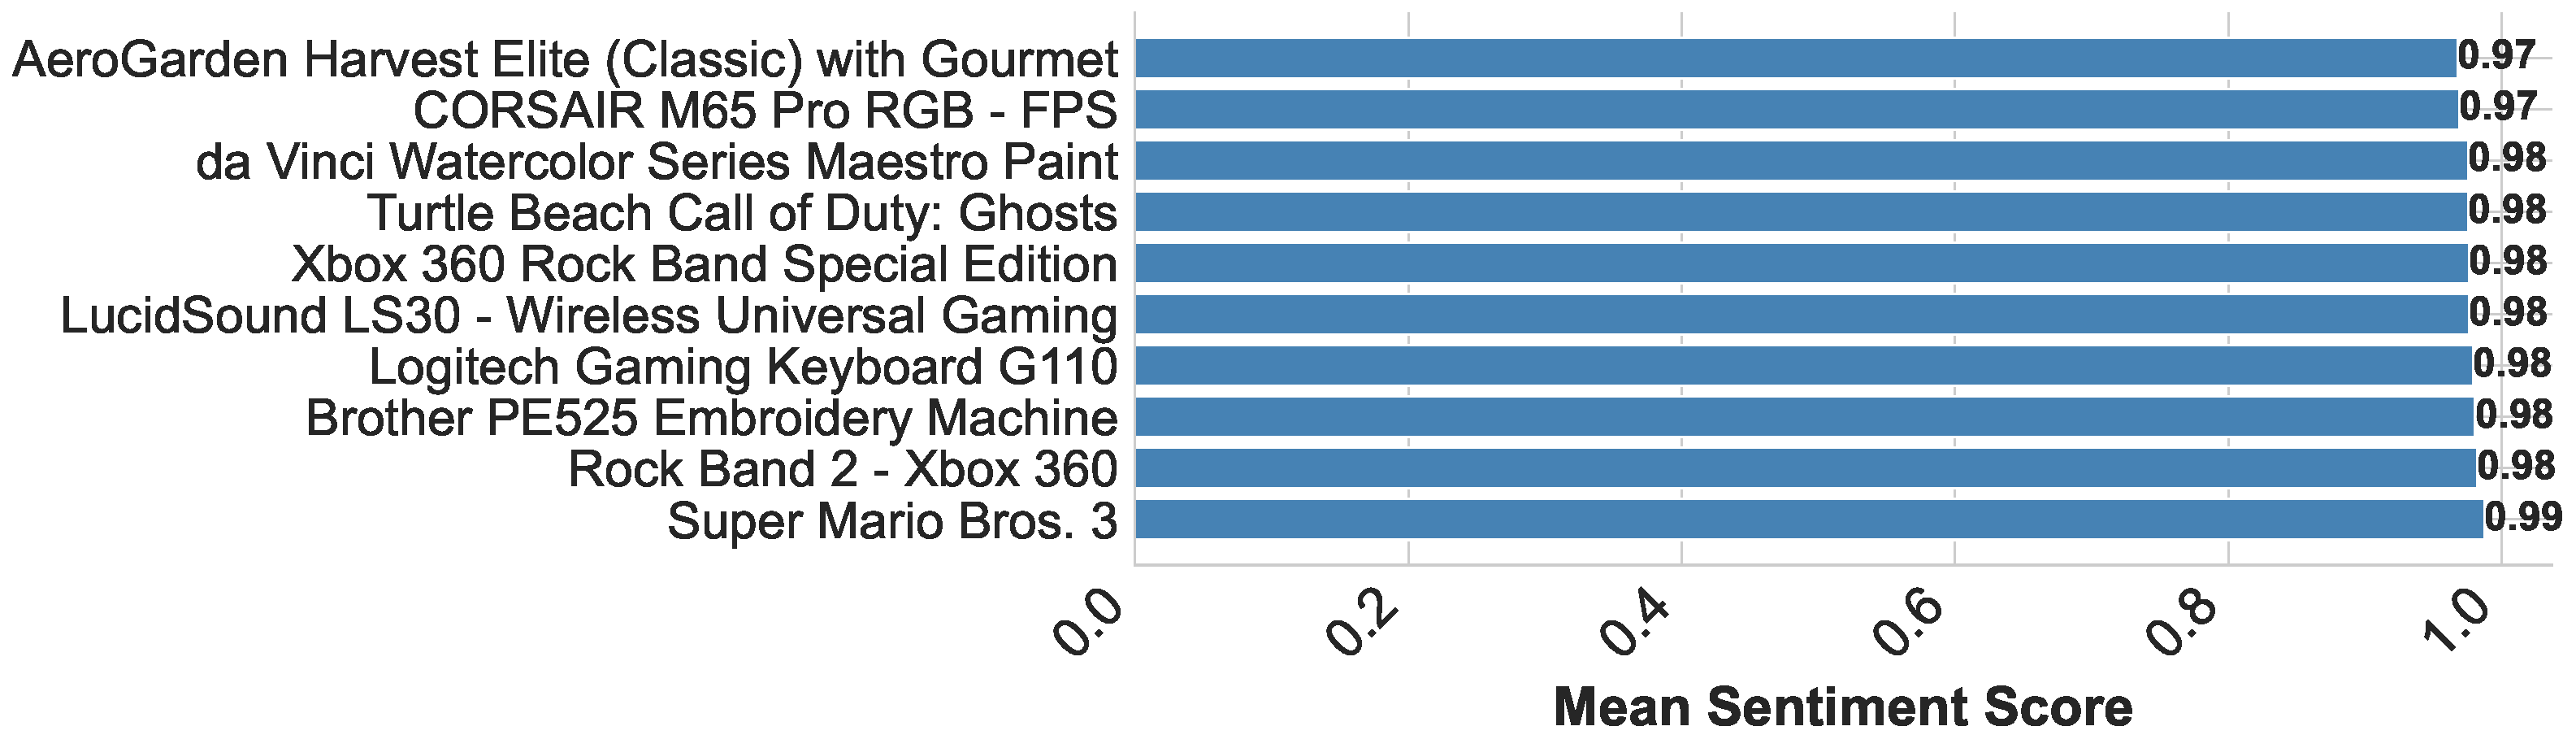
\includegraphics[width=0.98\textwidth]{Figures/Top_10_Products_Sentiments.pdf} % Adjust the file path and width as needed
    \caption{Top 10 Products Sentiments}
    \label{fig:top 10 products sentiments}
  \end{subfigure}
  \hfill
  \begin{subfigure}{\textwidth}
    \centering
    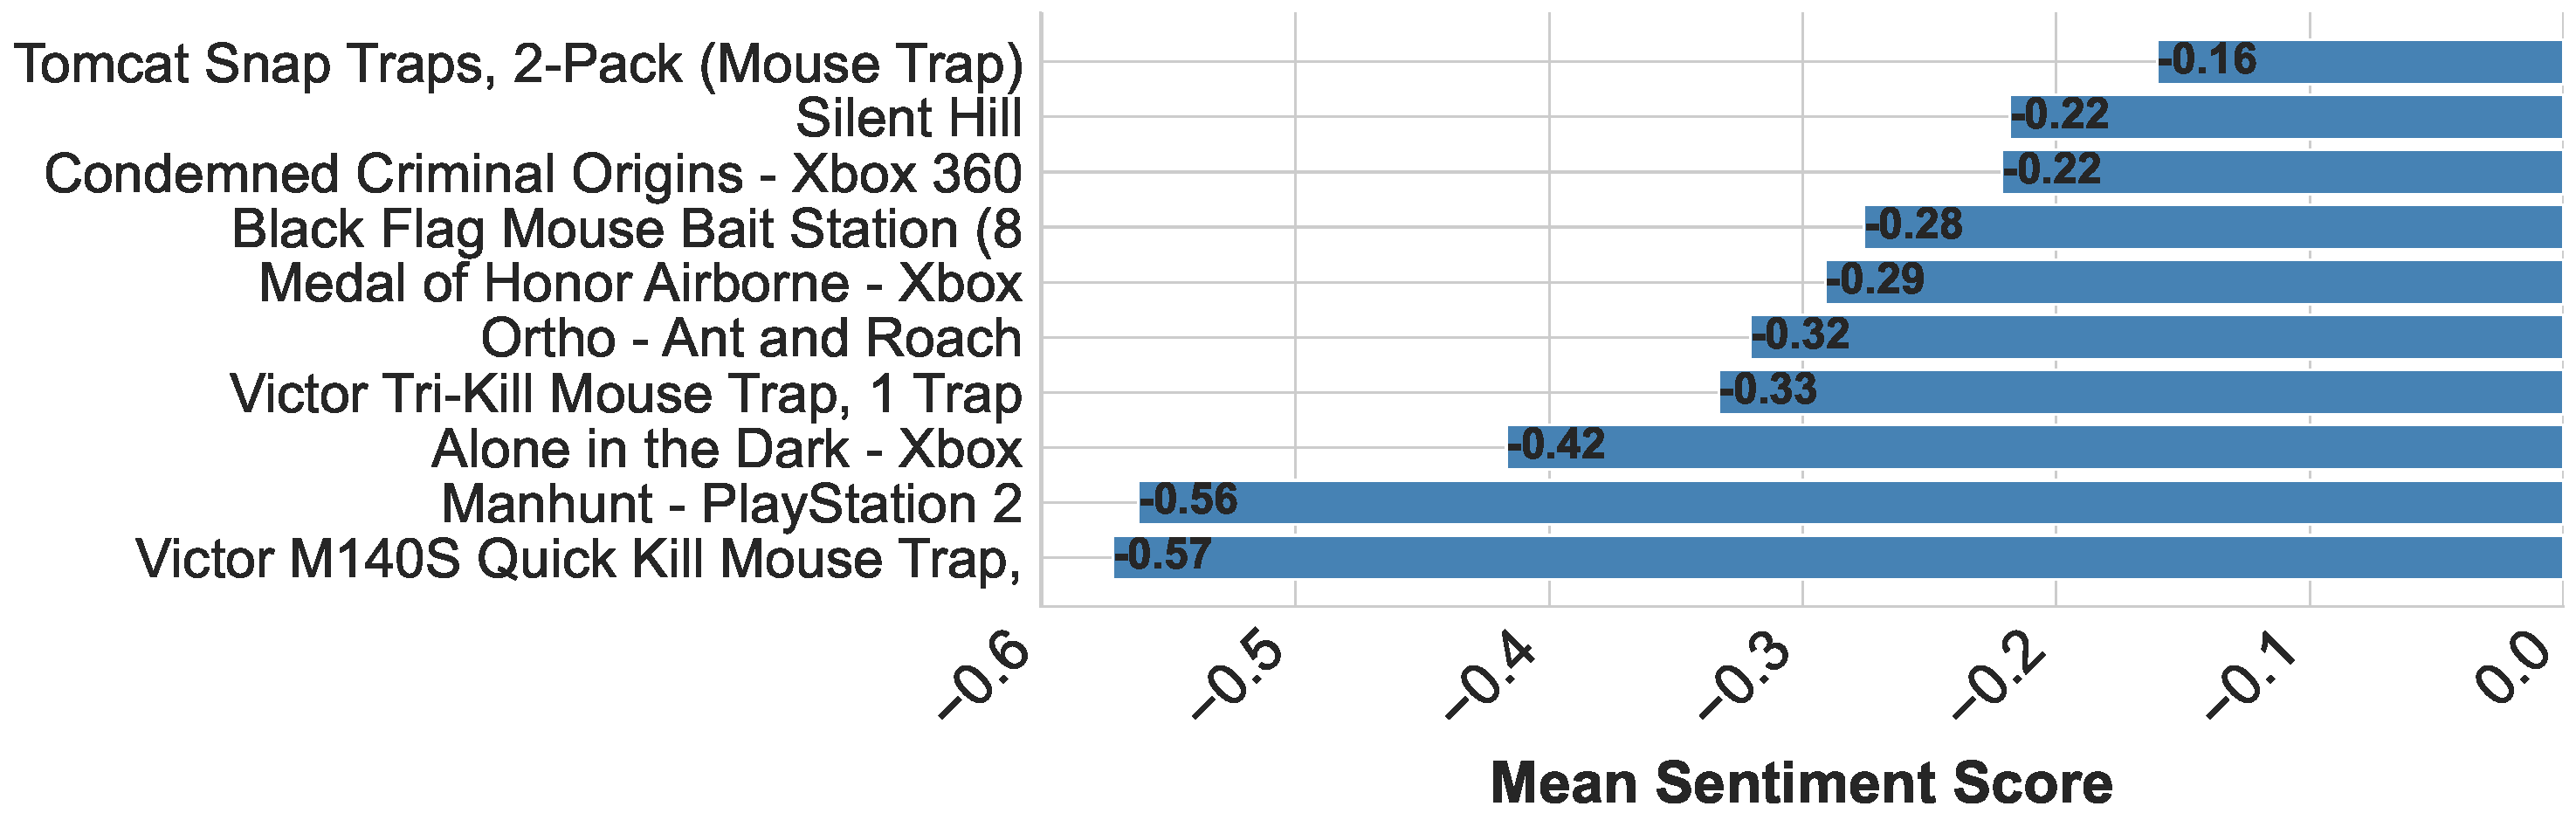
\includegraphics[width=0.98\textwidth]{Figures/Bottom_10_Products_Sentiments.pdf} % Adjust the file path and width as needed
    \caption{Bottom 10 Products Sentiments}
    \label{fig:bottom 10 products sentiments}
  \end{subfigure}
  \caption{Comparison of Sentiments for Top and Bottom 10 Products.}
  \label{fig:comparison_sentiments}
\end{figure}


\begin{table}[h]
  \centering
  \begin{tabular}{cccc}
      \hline
      \textbf{Product Title} & \textbf{Mean Rating} & \textbf{Count of Reviews} & \textbf{Mean Sentiment} \\
      \hline
      Super Mario Bros. 3                             &         4.733 &      15 &        0.987 \\
      Super Mario Bros. 3                             &         4.733 &      15 &        0.987 \\
      Rock Band 2 - Xbox 360                          &         4.6   &      15 &        0.982 \\
      Brother PE525 Embroidery Machine                &         4.692 &      13 &        0.981 \\
      Logitech Gaming Keyboard G110                   &         4     &      13 &        0.979 \\
      LucidSound LS30 - Wireless Universal Gaming     &         4.75  &      16 &        0.976 \\
      Xbox 360 Rock Band Special Edition              &         4.267 &      15 &        0.976 \\
      Turtle Beach Call of Duty: Ghosts               &         4.714 &      14 &        0.976 \\
      da Vinci Watercolor Series Maestro Paint        &         4.947 &      19 &        0.976 \\
      CORSAIR M65 Pro RGB - FPS                       &         4.8   &      15 &        0.969 \\
      AeroGarden Harvest Elite (Classic) with Gourmet &         4.75  &      16 &        0.968 \\
           \hline
  \end{tabular}
  \caption{Details about the Top 10 Products by Average Sentiment.}
  \label{tab:top 10 products statistics}
\end{table}


\begin{table}[h]
  \centering
  \begin{tabular}{cccc}
      \hline
      \textbf{Product Title} & \textbf{Mean Rating} & \textbf{Count of Reviews} & \textbf{Mean Sentiment} \\
      \hline
      Tomcat Snap Traps, 2-Pack (Mouse Trap) &         2.062 &      16 &       -0.16  \\
      Silent Hill                            &         4.56  &      25 &       -0.218 \\
      Silent Hill                            &         4.56  &      25 &       -0.218 \\
      Condemned Criminal Origins - Xbox 360  &         4.115 &      26 &       -0.221 \\
      Black Flag Mouse Bait Station (8       &         4.286 &      14 &       -0.276 \\
      Medal of Honor Airborne - Xbox         &         3     &      13 &       -0.291 \\
      Ortho - Ant and Roach                  &         4.357 &      14 &       -0.321 \\
      Victor Tri-Kill Mouse Trap, 1 Trap     &         3.615 &      13 &       -0.333 \\
      Alone in the Dark - Xbox               &         2.316 &      19 &       -0.417 \\
      Manhunt - PlayStation 2                &         3.895 &      19 &       -0.562 \\
      Manhunt - PlayStation 2                &         3.895 &      19 &       -0.562 \\
      Victor M140S Quick Kill Mouse Trap,    &         4.333 &      15 &       -0.572 \\
           \hline
  \end{tabular}
  \caption{Details about the Bottom 10 Products by Average Sentiment}
  \label{tab:bottom 10 products statistics}
\end{table}

The products with high sentiments (see Figure \ref{fig:top 10 products sentiments}) have received high positive feedback from users and furthermore, from Table \ref{tab:top 10 products statistics} we see that these products also have at least a mean rating of 4 (and more often than not closer to 5). This further reinforces the positive sentiment towards these products, indicating that they are well-received by users in terms of both ratings and review sentiments. We can say the same for the for bottom 10 products shown in Figure \ref{fig:bottom 10 products sentiments}  and Table \ref{fig:bottom 10 products sentiments} - these low mean sentiments achieved by these products reviews are also reflected in their mean ratings being mostly below 4.

To end off this visual analysis, Figure \ref{fig:correlation heat map sentiments} is a correlation heat map displaying the relationship between the various sentiment scores generated from AFINN, BING and VADER as well as the ratings and review word count. The goal here is to illustrate  whether there is a correlation between any of these sentiment scores with the ratings, and whether review length has a correlation with sentiments or ratings. From Figure \ref{fig:correlation heat map sentiments}, it is clear that VADER has the highest correlation with rating (0.32), suggesting a moderate positive relationship. This indicates that as the VADER sentiment score increases, the rating tends to increase as well. This is an important observation and was pivotal to our decision to use VADER as the sentiment analysis method of choice to generate sentiments to be used in our model. Specifically, AFINN and BING have lower correlations with rating (0.09 and 0.13 respectively), indicating weaker relationships with the rating.  Word count has a negative correlation with rating (-0.13), suggesting that longer reviews tend to have lower ratings - albeit the correlation is  weak. However, it has positive correlations with all three sentiment analysis techniques, with the highest being with AFINN (0.59). However, this is also an expected result, as AFINN (and BING) assign sentiment scores to each word in a review, and the cumulative score is influenced by the number of words \cite{haque2018sentiment}. Consequently, reviews with more words have a greater chance of containing positive words, resulting in higher sentiment scores. 

Ultimately, this section has provided us with a holistic understanding of the dataset's inherent structures and offers context-rich insights that will guide subsequent modelling, interpretation and discussions. However, before we detail the next steps, it is important to establish what data is used to train our models and what data is used to validate our models - this is studied in the next section. 

\begin{figure}[h]
  \centering
  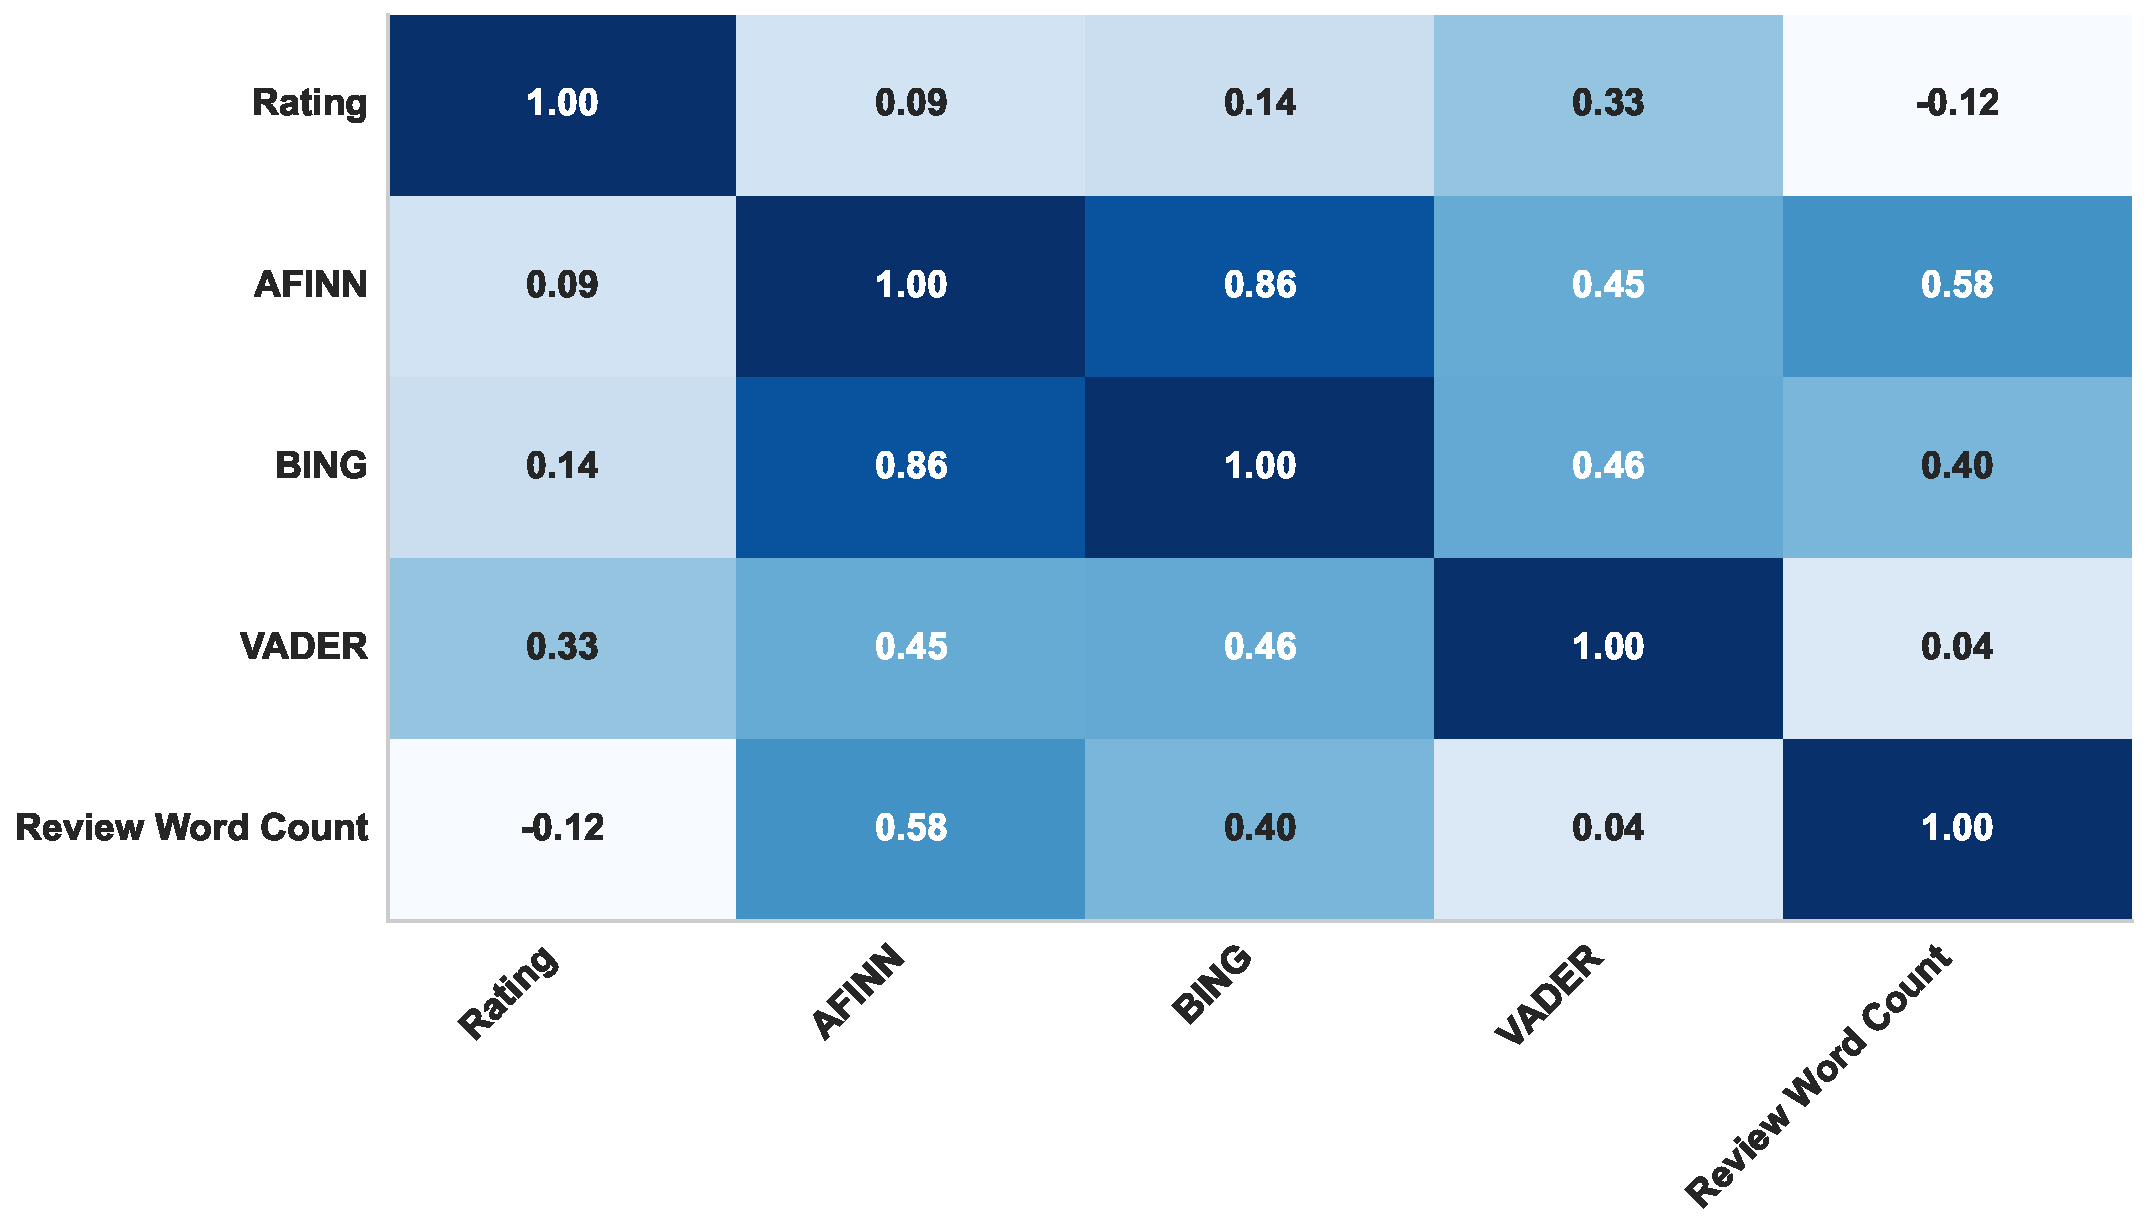
\includegraphics[width=0.9\textwidth]{Figures/correlation_between_ratings_sentiment_scores_review_length.pdf} % Adjust the width as needed
  \caption{Relationship Between Lexicon-Based Methods and Ratings.}
  \label{fig:correlation heat map sentiments}
\end{figure}


\section{Data Partitioning}
\label{sec:3 Data Partitioning}

When analysing a recommendation model, we are more concerned with its future performance on new (unseen) data, rather than its performance on past data \cite{witten2005practical}. In order to test future performance and estimate the prediction error, we must properly partition the original dataset into training and test subsets. This section outlines the data partitioning strategy employed for this thesis, considering the cleaned and transformed reviews dataset consisting of over 83 139 reviews.

Training data refers to the data that is used by one or more learning methods to develop the model and the test data is used to evaluate the quality of the model by giving the trained model this unseen (test) data \cite{witten2005practical}. The test set must be different and independent from the training set in order to obtain a reliable estimate of the true error \cite{witten2005practical}. It is important that performance is estimated on data which take no part in the formulation of the model. Some learning schemes, such as our case, need also a validation set in order to optimise the model parameters. In summary, to evaluate the performance of our recommender models, we need to train, validate (to optimise) and test our recommender model using different data. To do so, is not as simple as randomly allocating reviews (records) into three distinct sets. 

For recommender systems, the partitioning is performed by randomly selecting some ratings from all (or some of) the users. That is, for each user, we randomly select some ratings they have given and hide them, whilst keeping their remaining ratings in tact and to be used for training. The selected ratings constitute the test set, while the remaining ones are the training set. This method is called leave-$k$-out\footnote{method involves selecting a subset of $k$ ratings from the dataset as the test set, while the remaining ratings form the training set}. In \cite{sarwar2002incremental}, they split the dataset into 80\% training and 20\% test data following this leave-$k$-out approach. In \cite{herlocker1999algorithmic} the test set is made by 10\% of users: here only 5 ratings for each user in the test set are withheld. This leave-$k$-out approach is in fact also the method that we employ in our thesis. 

We opted to hide 3 random ratings from each user and allocate these to the test set, and hide another 2 (again random) ratings which were allocated to the validation set. We allocated the remaining reviews for the user to the training set. To further ensure the integrity of the partitioning process, we also ensured that the reviews for each user were randomly shuffled before allocating them to the respective subsets. This randomisation helps to mitigate any potential biases that may be present in the original dataset and ensures a representative distribution of user-item interactions across the subsets. We used a seed of 2207 to ensure reproducibility of the results. Note, there are other methods of splitting the dataset such as $k$-fold cross-validation\footnote{$k$-fold cross-validation divides the dataset into $k$ equally sized folds. The model is trained $k$ times, each time using $k-1$ folds for training and one fold for validation. The performance is then averaged over the $k$ iterations.}, however for our research we opted to use leave-$k$-out due to its simplicity and popularity in recommender research.

The choice for the partition was made to ensure that the recommender system is trained on a large enough dataset to capture the underlying patterns and relationships between users and items, whilst also ensuring that the test set is large enough to provide a reliable estimate of the model's performance. To that end, the training data, the largest partition of the data containing at least 7 reviews per user, comprises approximately 77.9\% of the dataset, or 64 799 reviews. The validation set comprises of approximately 8.8\% percent of the dataset (7 336 reviews). Finally, the test set is represented by approximately 13.2\% of the dataset (11 004 reviews). These datasets are summarised in Table \ref{tab:partition summary}.

\begin{table}[h]
  \centering
  \begin{tabular}{|l|l|l|l|}
  \hline
  \textbf{Dataset} & \textbf{Purpose} & \textbf{Number of Reviews} & \textbf{Proportion of Reviews} \\
  \hline
  Training & Training the model  & 64 799 & 77.9\% \\
  \hline
  Validation & Model validation  & 7 336 & 8.8\% \\
  \hline
  Testing & Model evaluation  & 11 004 & 13.2\% \\
  \hline
  \end{tabular}
  \caption{Dataset Partition}
  \label{tab:partition summary}
  \end{table}


  The partitioning of the dataset into training, validation, and test sets is crucial for achieving reliable and accurate results. It helps to evaluate the recommender system's performance on unseen data and provides an estimate of its effectiveness in real-world scenarios. The training set facilitates the learning of user preferences, the validation set aids in fine-tuning the model, and the test set provides an independent assessment of the system's performance. Having established this partitioning process, our data is ready to be used for our analysis. 




\section{Conclusion}
\label{sec:3 Conclusion}

In this chapter we have discussed a variety of aspects of the Amazon product review dataset, ranging from data collection and preparation to exploratory data analysis and data partitioning for recommender systems. 

Specifically, in Section \ref{subsec:3 Amazon Review Dataset}, we provided some background and context on the Amazon Product Reviews dataset, which we have chosen for this thesis. In this same section we also dived into the details of the type of user feedback that we have in the dataset and explained that we are using explicit feedback provided through numerical ratings and review text variables. In section \ref{sec:3 Variable Description}, we provided a brief overview of the variables in the dataset and gave some descriptions of these. 

The data that consists of over 75 million reviews over a 22-year period. Through data management and filtering (see Section \ref{sec:3 Data Collection and Preprocessing}), we were able to extract a subset of the data that contains 91 235 reviews from 3801 unique users and 3283 unique products. In this same section, we also explained in detail the preprocessing steps taken to ready the data for further analysis, which included handling of nulls and duplicates amongst other steps. Subsection \ref{subsec:3 Text Analysis and Cleaning} and \ref{subsec:3 Sentiment Analysis} summarised the work done to analyse and clean the textual data - the user review text. These sections outlined the text cleaning steps taken from normalising  to lemmatising the review text. We also covered what sentiment analysis is (see Section \ref{subsec:3 Sentiment Analysis}) and why we opted for the VADER lexicon-based approach to generate the sentiment feature for the dataset. At this stage we had filtered our dataset to 83 139 reviews in the dataset, where we had 3668 unique users and 3249 unique products 

Sections \ref{sec:3 Data Summary} and \ref{sec:3 Trends and Patterns} provided a brief high level visual summary of the dataset from different angles, looking at user engagement, review text and ratings data. We looked at the distributions and identified any trends in the data. Over the entire cleaned data set of reviews (approximately 83 139 reviews), the average ratings are 4.4 - where the ratings are on a five-point scale. We also identified that the general sentiment of users vary, however they are majority positive. Lastly, we outlined the method of partition of our dataset in Section \ref{sec:3 Data Partitioning}. Data partitioning is a pivotal step in the development and evaluation of recommender systems, serving to gauge the system's ability to generalise to unseen user-item interactions. We opted for the leave-$k$-out approach where we simply, hid or removed 5 ratings at random from each user and allocated 2 of those hidden ratings to a validation set and 3 of them to a testing set, the balance of the ratings were used as the training set. 

As we transition to the next chapter on methodology, we build upon this foundational understanding of the dataset to look into the intricacies of our approach for building and evaluating recommender systems.
